\documentclass[12pt,a4paper]{report}
\usepackage[top=2.5cm, bottom=2.5cm, left=2.5cm, right=2.5cm]{geometry}

% Différentes options pour la classe :
% - taille de la fonte    : 10pt, 11pt, 12pt
% - recto ou recto-verso    : oneside, twoside
% - stade de développement    : draft, final

\usepackage[french]{babel}
% \usepackage[english]{babel}
%\usepackage[latin1]{inputenc}    % Pour utiliser les lettres accentuées

%\usepackage[utf8]{inputenc}%           gestion des accents (source)
\usepackage[T1]{fontenc}%              gestion des accents (PDF)
%\usepackage[francais,english]{babel}%          gestion du français
\usepackage[utf8]{inputenc}
\usepackage{textcomp}%                 caractères additionnels

\usepackage[pdftex]{graphicx}
\usepackage{setspace}
\onehalfspacing
\usepackage{hyperref}
\usepackage[french]{varioref}
\usepackage{fancyhdr}
\usepackage{color}
\usepackage{colortbl}
\usepackage{amsmath}
\usepackage{ifpdf} % part of the hyperref bundle
\usepackage{array} 
\usepackage{tabularx}
\usepackage{tabularray}
\usepackage{cellspace}
\usepackage{longtable}
\usepackage{multirow}
\usepackage{enumitem}
\usepackage{etoc}
\usepackage{geometry}
\usepackage[explicit]{titlesec}
\usepackage{xhfill}
\usepackage{pdfpages}
\usepackage{titlesec}
\usepackage{xcolor}
\usepackage{graphicx}
\usepackage{longtable}
\usepackage{booktabs}
\usepackage{caption}
\usepackage{enumitem}

%\usepackage{abstract}
\newcolumntype{c}[1]{>{\centering\let\newline\\\arraybackslash\hspace{0pt}}m{#1}}
\newcolumntype{l}[1]{>{\raggedright\let\newline\\\arraybackslash\hspace{0pt}}m{#1}}
\newcolumntype{r}[1]{>{\raggedleft\let\newline\\\arraybackslash\hspace{0pt}}m{#1}}


 % set fonts for nicer pdf view
 \IfFileExists{lmodern.sty}{\usepackage{lmodern}}{}


\pagestyle{fancy}
\fancyhead[L]{\nouppercase\leftmark} %pour afficher le nom du chapitre à gauche
\fancyhead[C]{}
\fancyhead[R]{} %pour afficher le nom de la section à droite

\usepackage{float}

\fancyfoot[L]{}
\fancyfoot[C]{}
\fancyfoot[R]{\textbf{\thepage}}







% Début du document
\begin{document}

% %%%%%%%%%%%%%%%%%%%%%%%%%%%%%%%%%%%%%%%%%
% University Assignment Title Page 
% LaTeX Template
% Version 1.0 (27/12/12)
%
% This template has been downloaded from:
% http://www.LaTeXTemplates.com
%
% Original author:
% WikiBooks (http://en.wikibooks.org/wiki/LaTeX/Title_Creation)
%
% License:
% CC BY-NC-SA 3.0 (http://creativecommons.org/licenses/by-nc-sa/3.0/)
% 
% Instructions for using this template:
% This title page is capable of being compiled as is. This is not useful for 
% including it in another document. To do this, you have two options: 
%
% 1) Copy/paste everything between \begin{document} and \end{document} 
% starting at \begin{titlepage} and paste this into another LaTeX file where you 
% want your title page.
% OR
% 2) Remove everything outside the \begin{titlepage} and \end{titlepage} and 
% move this file to the same directory as the LaTeX file you wish to add it to. 
% Then add \input{./title_page_1.tex} to your LaTeX file where you want your
% title page.
%
%%%%%%%%%%%%%%%%%%%%%%%%%%%%%%%%%%%%%%%%%





\newcommand{\HRule}{\rule{\linewidth}{0.5mm}} % Defines a new command for the horizontal lines, change thickness here

 % Center everything on the page
 
%----------------------------------------------------------------------------------------
%	HEADING SECTIONS
%----------------------------------------------------------------------------------------
\begin{center}
    


\begin{minipage}[l]{0.8\columnwidth}
\centering
\large
\textbf{\textsc{Ministère de l'Enseignement Supérieur et de la Recherche Scientifique}}\\
\medskip 
\textbf{\textsc{Université de Manouba}}\\
\medskip 
\textbf{\textsc{Institut supérieur des Arts Multimédias}}

\vspace{0.5cm}
\includegraphics[width=0.6\columnwidth]{logo-isamm.jpeg}
\end{minipage}
\hfill


\vskip1cm
\textsc{\large Mémoire de fin d'études}\\[0.5cm] % Minor heading such as course title\\

\textbf{Préparé en vue de l'obtention du diplôme ..}

\vskip1cm%

%----------------------------------------------------------------------------------------
%	TITLE SECTION
%----------------------------------------------------------------------------------------

\HRule \\[0.4cm]
{ \LARGE \bfseries Nom du projet}\\[0.3cm] % Title of your document
\HRule \\[1cm]


\textit{Réalisé par}\\
\vskip0.5cm
\textsc{\large Aymen Mohsni}\\[0.5cm] % Minor heading
\textsc{\large Mohsni Aymen}\\[0.5cm] % Minor heading

\vspace{1cm}
\textit{Encadré par}\\ 
\vskip0.5cm
\textsc{\large M./Mme : Prénom Nom - ISAMM}\\[0.5cm] % Minor heading
\textsc{\large M./Mme : Prénom Nom - Société d'accueil}\\[0.5cm] % Minor heading

\vspace{1cm}
{\large Année Universitaire: 2022 - 2023}\\[1cm] 




%\end{document}

\end{center}

% \include{garde_fin1}


% \includepdf[pages={1}]{images/page de garde t4g.pdf}


\newpage

\pagenumbering{roman}
\renewcommand{\thepage}{}

% \chapter*{Dedication }
%\addcontentsline{toc}{chapter}{Dédicaces }

\begin{center}

\begin{minipage}[c]{1\columnwidth}

{\large 
\vskip0.25cm

\centering

\begin{large}
I dedicate this work...

\vspace{0.5cm}

To my beloved late father, \textbf{Hachmi}, whose memory continues to inspire me. Although you left this world, your love and guidance have shaped the person I have become.

\vspace{0.5cm}

To my dear mother, \textbf{Jamila}, your unwavering love, support, and sacrifices have been a source of strength throughout my journey. I am forever grateful for your unwavering dedication, which has inspired me to push boundaries and strive for excellence.

\vspace{0.5cm}

To my brothers, \textbf{Hichem} and \textbf{Mohamed Ali}, thank you for always being there for me. Your support, encouragement, and camaraderie have been invaluable. You are my pillars of strength.

\vspace{0.5cm}

To my friends, \textbf{Hamed Chamkhi} and \textbf{Abdelkhalek Ziraoui}, thank you for your unwavering friendship, support, and countless memorable moments. Your presence has made this journey all the more meaningful.

\vspace{0.5cm}

To my dear family,
No words can fully express how much you mean to me. Your presence in my life is invaluable, and I pray that God blesses you with happiness and good health

\end{large}

}


\end{minipage}

\end{center}

\vskip1.5cm
\begin{flushright}\LARGE
\bf{Moetez Theiri}
\end{flushright}








% \chapter*{Dédicaces }
%\addcontentsline{toc}{chapter}{Dédicaces }

\begin{center}

\begin{minipage}[c]{1\columnwidth}

{\large 
\vskip1cm

\centering
Je dédie ce projet à...
}


\end{minipage}

\end{center}

\vskip1.5cm
\begin{flushright}\LARGE
\bf{Binome2}
\end{flushright}








% \chapter*{Acknowledgement }
%\addcontentsline{toc}{chapter}{Remerciement }

\begin{large}
Upon the conclusion of this endeavor, I wish to extend my gratitude to Allah for bestowing upon me the strength, determination, and patience necessary to accomplish this work.

\vspace{1.5cm}

I would like to express my sincere appreciation to \textbf{Mrs. Ines Ben Hassine}, my supervisor, for her invaluable guidance, kindness, and support throughout the realization of my project.

\vspace{1.5cm}

I would also like to acknowledge and thank \textbf{Mrs. ACHOURA Najoua} for the esteemed role of moderating the jury, and \textbf{Mrs. Ben Ahmed Afef} for graciously accepting the responsibility of examining this report.

\vspace{1.5cm}

Lastly, I am deeply grateful to my family for their unwavering support and encouragement throughout this journey.
\end{large}

\vskip1.5cm
\begin{flushright}\LARGE
\bf{Moetez Theiri}
\end{flushright}

\renewcommand{\contentsname}{Table of Contents}
\tableofcontents     % Table of Contents

\renewcommand{\listfigurename}{List of Figures}
\listoffigures        % Liste des figures

\renewcommand{\listtablename}{List of Tables}
\listoftables        % Liste des tableaux
%%\addcontentsline{toc}{chapter}{Acronymes}

\chapter*{Liste des acronymes}
\begin{acronym}
\Large
\acro{SEO} :  {\emph{Search Engine Optimization}}

\acro{RDV} :  {\emph{Rendez-Vous }}
\end{acronym}
\normalsize

\newpage
\pagenumbering{arabic}

\chapter*{General Introduction}
\markboth{General Introduction}{} %pour afficher l'entete
\addcontentsline{toc}{chapter}{General Introduction}

\begin{large}
Throughout history and, across cultures communication has always played a role in human life. From times when people carved messages on stone tablets to today's era of global connectivity the need to communicate has remained constant. The evolution of communication technologies from the telegraph to \textbf{5G} networks has not made it easier to connect with others but has also driven innovation and progress pushing human civilization forward in terms of knowledge and connection. The telecommunications sector sees millions of dollars exchanged daily making it a fertile ground for investment and economic growth due to its demand and rapid technological advancements. Governments worldwide implement frameworks of regulation to ensure fairness, efficiency and equal access for all parties involved in telecommunications. These regulations aim to maintain the integrity of the telecommunications ecosystem and protect the rights of consumers, as industry players. In this changing landscape where innovation meets necessity, regulations serve as pillars of stability and fairness guaranteeing that connectivity continues to benefit societies by empowering them.


\vspace{0.5cm}

Being a student of computer science driven by a passion to facilitate the life of  every day's users I have been given an amazing opportunity. With a commitment to fairness, my task is to create a mobile application that will act as a bridge of information seamlessly connecting customers with the intricate world of telecommunications in their country. This noble mission aims to empower users by providing insights into networks and telecommunication  services fostering relationships, among all involved parties. Through the development of this app my goal is to close the divide ensuring that every user possesses the knowledge and tools to navigate the digital landscape confidently and clearly.


\vspace{0.5cm}

This report is composed from  four chapters in which , I demonstrate the whole process that I went through to realise this project:



\begin{itemize}
    \item The first chapter \textbf{"Preliminary Study"}: In this chapter I will present the host firm ,cover the  general frame of the project  and its functional and non-functional requirements , also it will contain the explanation of some terminologies used through the whole project , beside the chosen project management approach , a demonstration of the software arsenal used along the project and lastly the implemented architecture .
\end{itemize}

% \vspace{0.5cm}

\begin{itemize}
    \item The second chapter "" Mobile Application Development: The third and fourth chapter dive into the meticulous creation and implementation of the mobile application. Through iterative development, we detail each sprint's progress, covering facets of user interface, user experience, backend integration, and testing.
\end{itemize}


% \vspace{0.5cm}


This journey showcases the synergy of innovation and execution, demonstrating the potential of digital solutions in enhancing event engagement. With a focus on user-centered design and agile development, we're proud to present a solution that bridges the gap between event organizers and enthusiasts, ushering in a new era of seamless event experiences.


\end{large}












\titleformat{\chapter}[block]
{\filcenter\bfseries\Huge}
{\xrfill[0.4ex]{5pt}\ \thechapter.\ \xrfill[0.4ex]{5pt}}
{0pt}
{\xrfill[0.4ex]{5pt}\ \MakeUppercase{#1}\ \xrfill[0.4ex]{5pt}}


\titleformat{\chapter}[block]
{\filcenter\bfseries\Huge}
{\xrfill[0.4ex]{5pt}\ \thechapter.\ \xrfill[0.4ex]{5pt}}
{0pt}
{\xrfill[0.4ex]{5pt}\ \MakeUppercase{#1}\ \xrfill[0.4ex]{5pt}}


\chapter*{Chapter 1}
\markboth{Chapter 1: Preliminary study}{1 Preliminary study} %pour afficher l'entete
\addcontentsline{toc}{chapter}{1 Preliminary study}




\setcounter{chapter}{1}


\etocsettocstyle{\subsection*{Plan}}{}
\vspace{0.25cm}

\setcounter{tocdepth}{1}
\headrule{
\vspace{0.5cm}

\begin{center}
    \textsc{\textbf {\Huge Preliminary study}} 
\end{center}
}
\headrule


\localtableofcontents
\newpage


%\end{chapter1}
\section*{Introduction}
Through this chapter we'll have a clear vision about the host company , its filed of activity  and its artifacts beside the global context of my internship .Also in this chapter we'll shed light on the encountered problematic and some existing solutions in the market and their limitations, then we'll have a comparative study of project management methodologies to come up with a suitable one for the needs of this project .


\section{Presentation of host organization}

This internship took place at Business Intelligence For Telecommunication, a TIC (Information and Communication Technology) company, founded in 2010, provides reliable and comprehensive solutions for the study, control, and monitoring of the quality of service of cellular networks. BI4T operates in various parts of the value chain of TIC (Information and telecommunication Technology) such as radio, architectural design, and software development. located at Tunis.

It was done over an extended  period of four months, from 1\textsuperscript{st}
February 2024 to 31 May 2024.

\begin{figure}[H]
    \centering
    
\includegraphics[height=4.5cm]{images/chap1/LOGO_BI4T.png}
    \caption{BI4T Logo} \cite{BI4T}
    \label{fig:enter-label}
\end{figure}

\section{BI4T legacy}
Throughout a span of 14 years BI4T has gained an understanding of the frameworks and market dynamics in the telecommunications sector. This vast experience has allowed them to navigate the realm of compliance while also leveraging emerging market trends. A standout accomplishment, on this journey is the creation of the QoS Tracker, a tool that transforms how customers monitor and manage telecommunications processes. With its range of features the QoS Tracker not meets but surpasses our clients requirements offering unmatched insights, into the service quality delivered by telecommunications networks.

\begin{figure}[H]
    \centering
    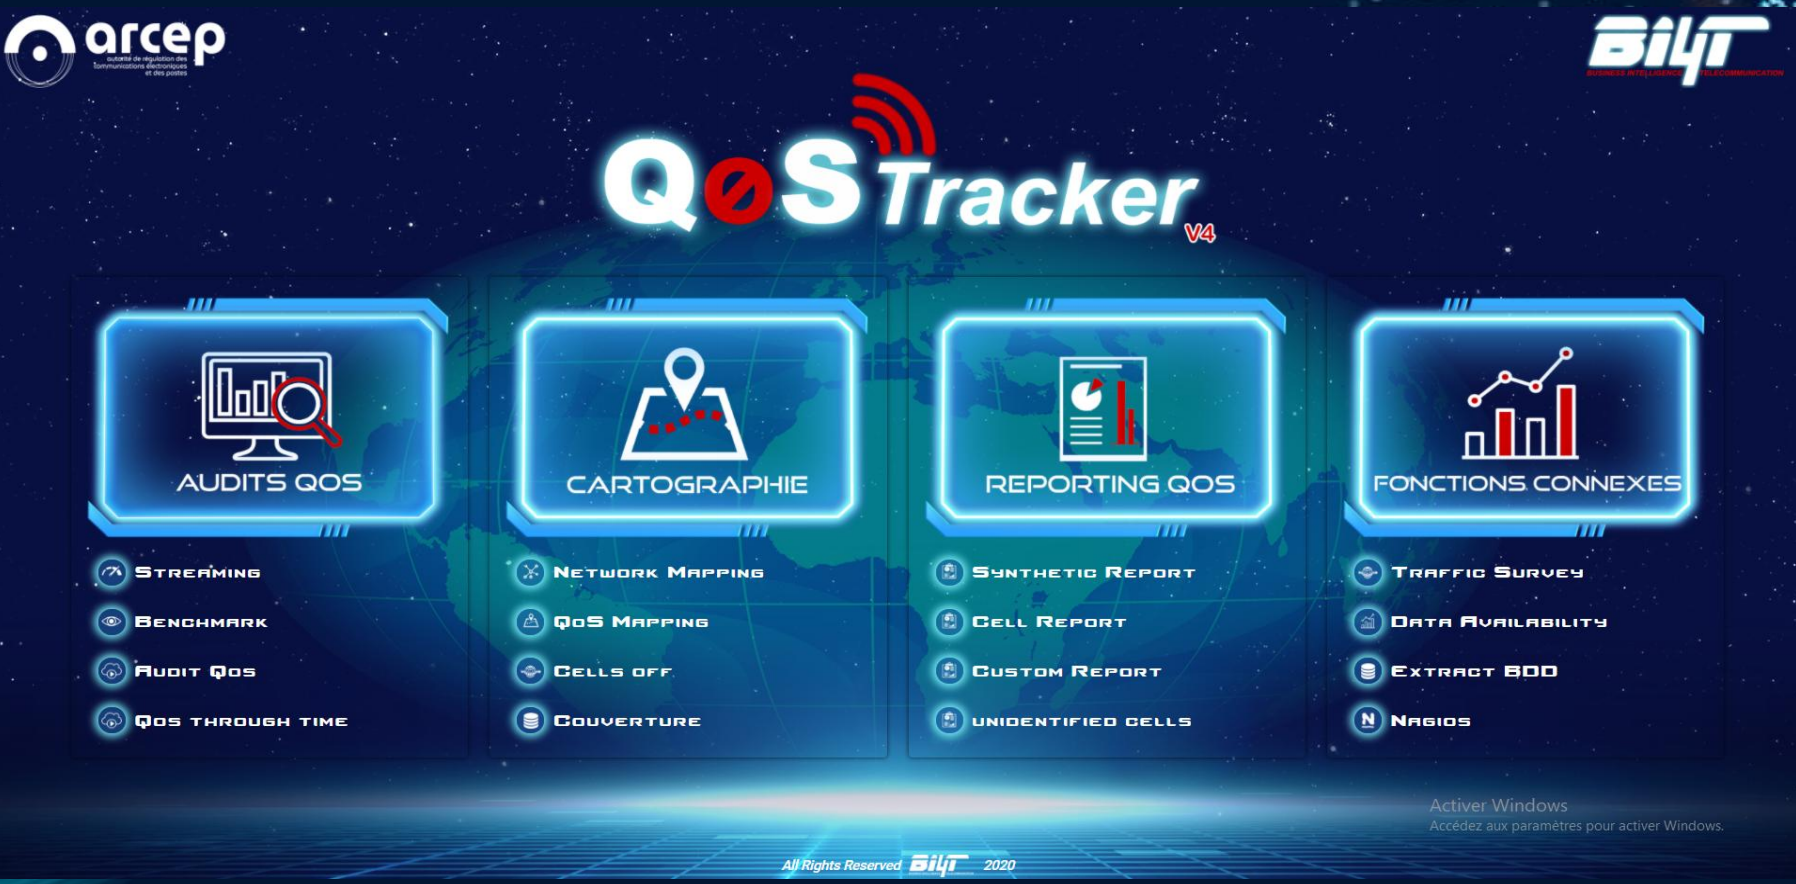
\includegraphics[height=8cm]{images/chap1/QoStrackerV4.png}
    \caption{QoS tracker interface}
    \label{fig:enter-label}
\end{figure}
\begin{figure}[H]
    \centering
    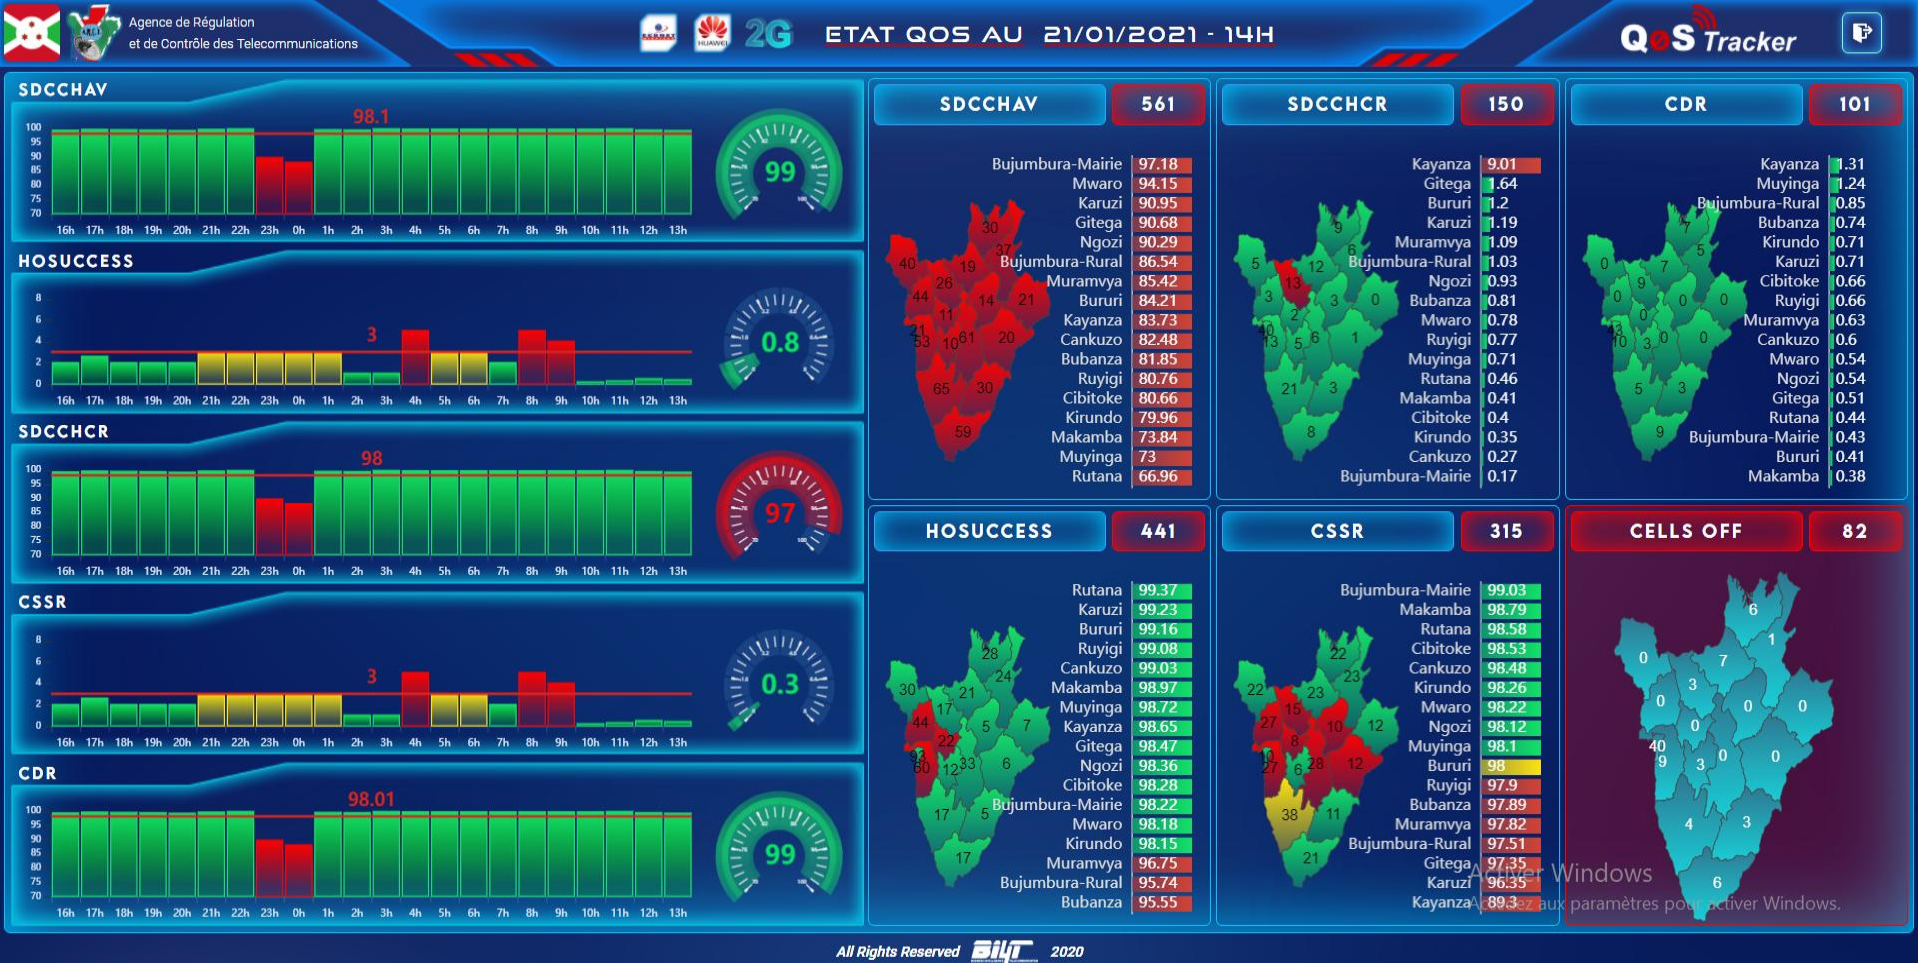
\includegraphics[height=8cm]{images/chap1/QoStrackerV4_1.png}
    \caption{QoS tracker interface}
    \label{fig:enter-label}
\end{figure}




\section{Telecommunication regulation process}
Our contemporary landscape of electronic communication is imbued with layers of significance and confidentiality, rendering it invaluable in its essence. Understanding the weight of this reality, governments worldwide have instituted a comprehensive regulatory regime to oversee telecommunication companies and operators. Through the enactment of laws and the establishment of regulatory bodies, these governments seek to create a framework that balances the imperatives of security, privacy, and accessibility. The power of monitoring vested in these regulatory entities serves as a linchpin for ensuring compliance and upholding the integrity of the telecommunication process.
As a two major axis of this regulation , governments instances often emphasize the importance of ensuring that users privacy is respected, as maintaining a fair level of quality of service (QoS) and quality of experience (QoE). 
% not done yet need one more img to describe the process + some points to describe each step
The result of this process is determined by the calculation of some KPI :
\begin{itemize}
    \renewcommand\labelitemi{\textbf{\Huge .}}
    \item  An OMC server collects raw data that contains some counter values from operator site and send them  to a DCS sever
    \item  Every DCS server organize the coming files in group based on equipment type and network generation then sends them to a dedicated server in the regulator site via a secure connection 
    \item The frontal servers then perform the processing and calculation of the provided counters based on a documentation given by the operator to have the final values of the KPIs 
    \item The frontal servers save raw data and aggregated data to the database 
    \item Web client consume the aggregated data to perform visualization and extract value from it 
    \end{itemize}

\begin{figure}[H]
    \centering
    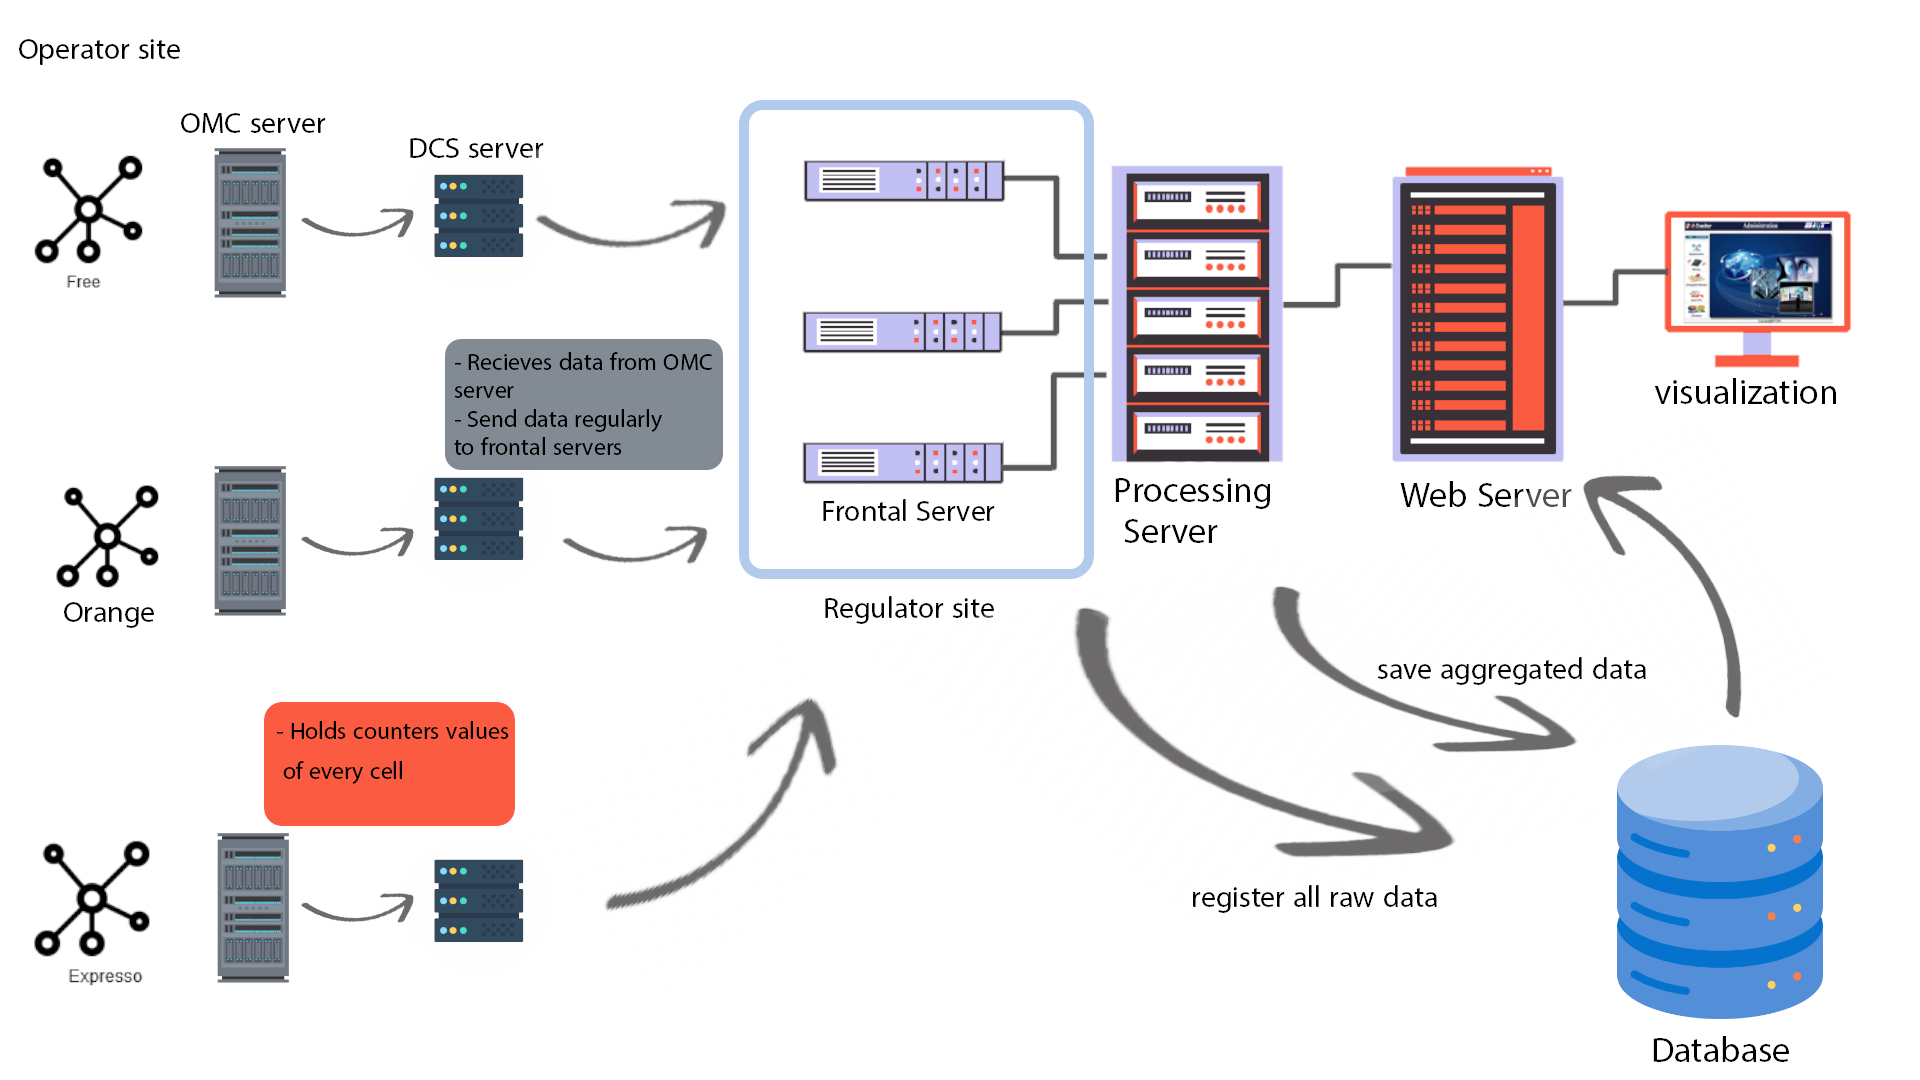
\includegraphics[height=10cm]{images/chap1/archi_1.png}
    \caption{Regulation process schema}
    \label{fig:enter-label}
\end{figure}






\section{Problematic}
BI4T offers a specialized software package tailored for professional utilization, which inherently relies on the expertise of regulatory technicians for its effective implementation. However, the absence of skilled subscribers poses a significant risk to its efficacy. In response to the imperative of transparency and efficient information dissemination, regulatory bodies frequently opt to complement their software package with a companion mobile application. This strategic choice aims to bridge potential gaps caused by subscriber absence. Our responsibility involves the development of this mobile channel, ensuring its accessibility and user-friendliness across all user demographics. Through this application, users gain access to a comprehensive repository of relevant information, facilitating the continuous monitoring of network conditions. Additionally, it serves as a platform for users to offer feedback and make inquiries, fostering a collaborative environment conducive to the enhancement of telecommunications services.


% \section{Proposed Solution}
\newpage
\section{Existing  Solutions}
A lot of companies have treated the quality of service tracking topic with applications such as:


\subsection{nPref speed test}
\textbf{nPerf}   brings you the best and the fullest mobile connection quality measurement tool up to 1 Gb/s speeds!

Full QoS test: In few seconds, test your bitrate speed, latency, browsing speed and video streaming quality on your mobile device.
Comparison function: Compare your results with those of others users and for each provider with a real time barometer.
Interactive map: Check network coverage and carriers performances in your area (in USA : AT\&T, Sprint, T-Mobile, Verizon Wireless).\cite{nPerf}
% \cite{https://play.google.com/store/apps/details?id=com.nperf.tester&hl=en&gl=US}.
\begin{figure}[H]
    \centering
    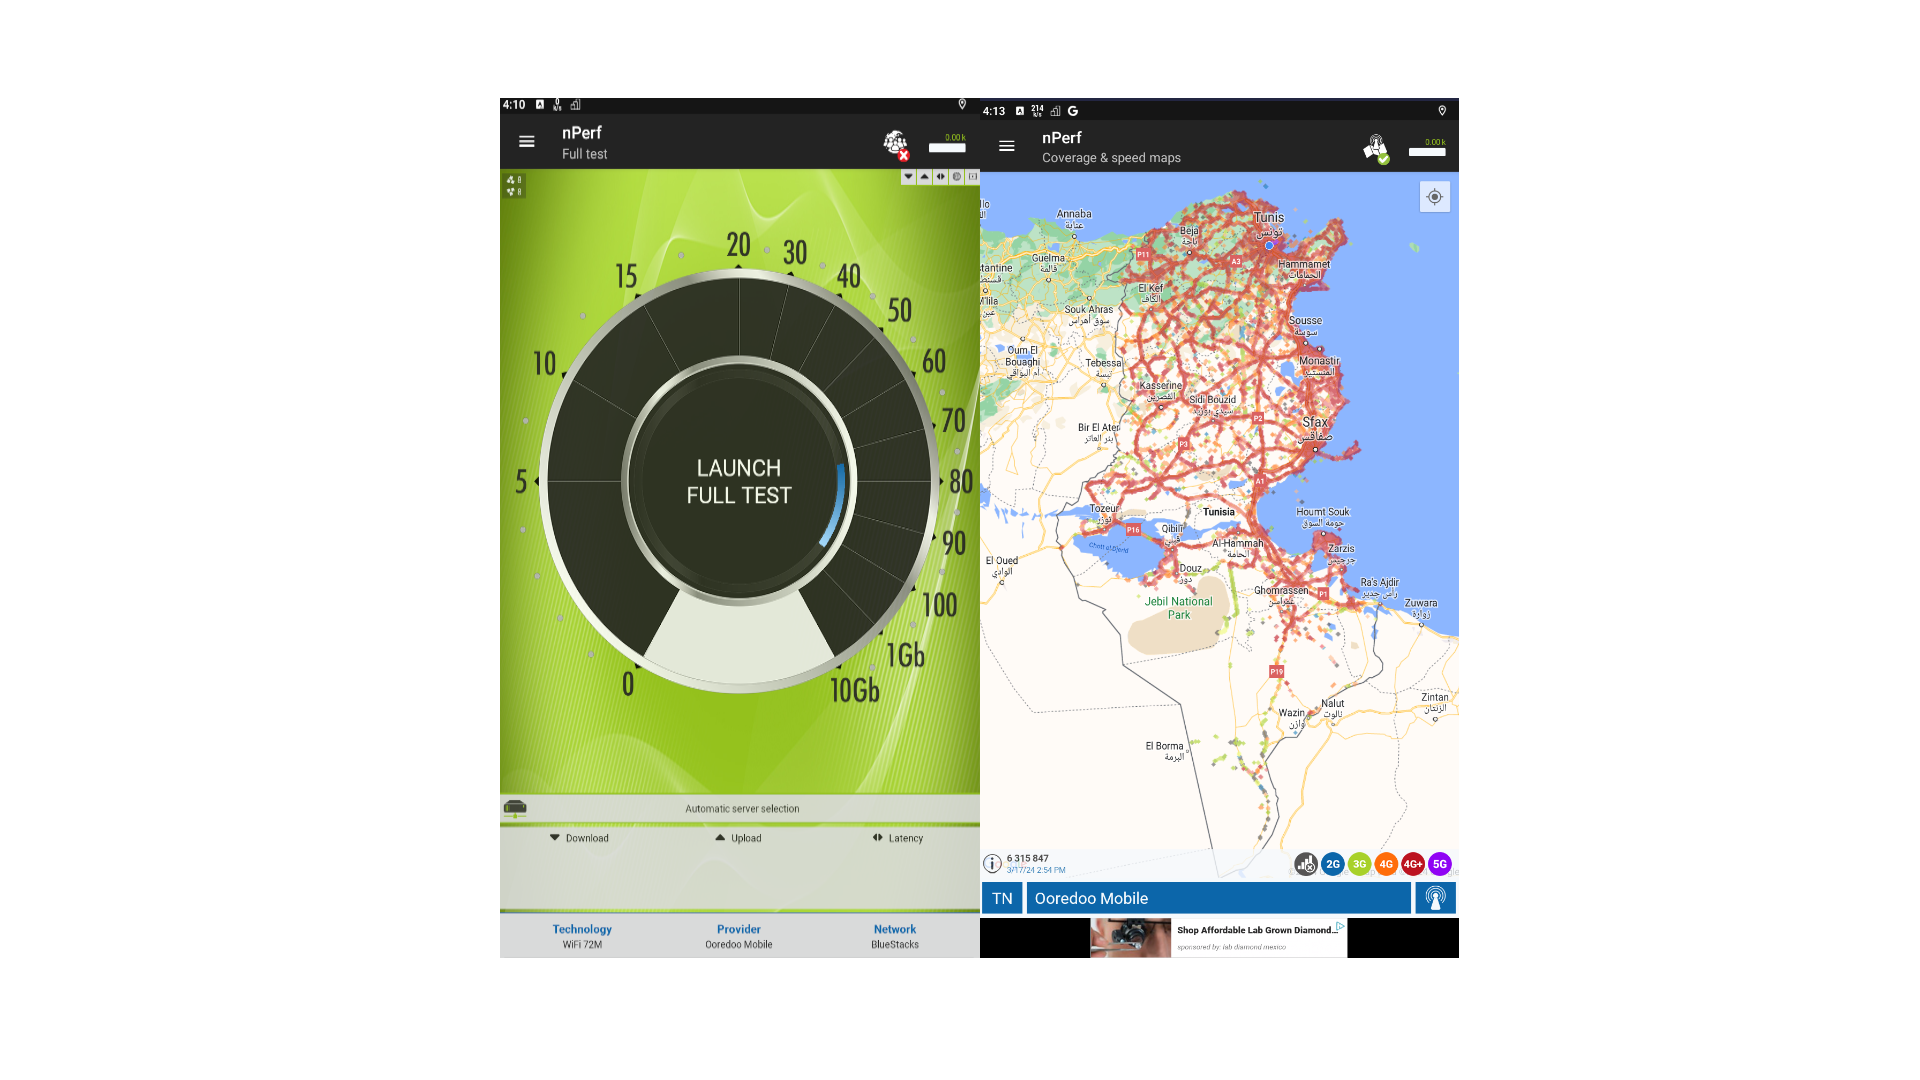
\includegraphics[height=12cm]{images/chap1/nPref.png}
    \caption{nPref speed test demo}
    \label{fig:enter-label}
\end{figure}
\textbf{nPref} mobile app comes up with :
\begin{itemize}
    \renewcommand\labelitemi{\textbf{\Huge .}}
    \item  Decent User Interface
    \item  Speed test section
    \item Coverage map 
  
\subsubsection*{Advantages}
\begin{itemize}
\renewcommand\labelitemi{\textbf{\Huge .}}
    \item Fullest mobile connection quality measurement tool up to 1 Gb/s speeds
    \item User friendly interface
\end{itemize} 

\subsubsection*{Disadvantages}
\begin{itemize}
\renewcommand\labelitemi{\textbf{\Huge .}}
    \item The data is often outdated 
    \item Without subscription user forced to see adds
    \item The data source in unknown
\end{itemize} 
\end{itemize}

% 2nd
\subsection{RfBenchmark}
\textbf{RfBenchmark}  Mobile application RFBENCHMARK allows measurements of radio coverage provided by mobile operator and testing of Internet Connection Quality for different Radio Access Technologies (RAN), such as: GSM, 3G, LTE, WIFI.\cite{RFBenchmark}
% \cite{https://rfbenchmark.com/en/application-2/}.
\begin{figure}[H]
    \centering
    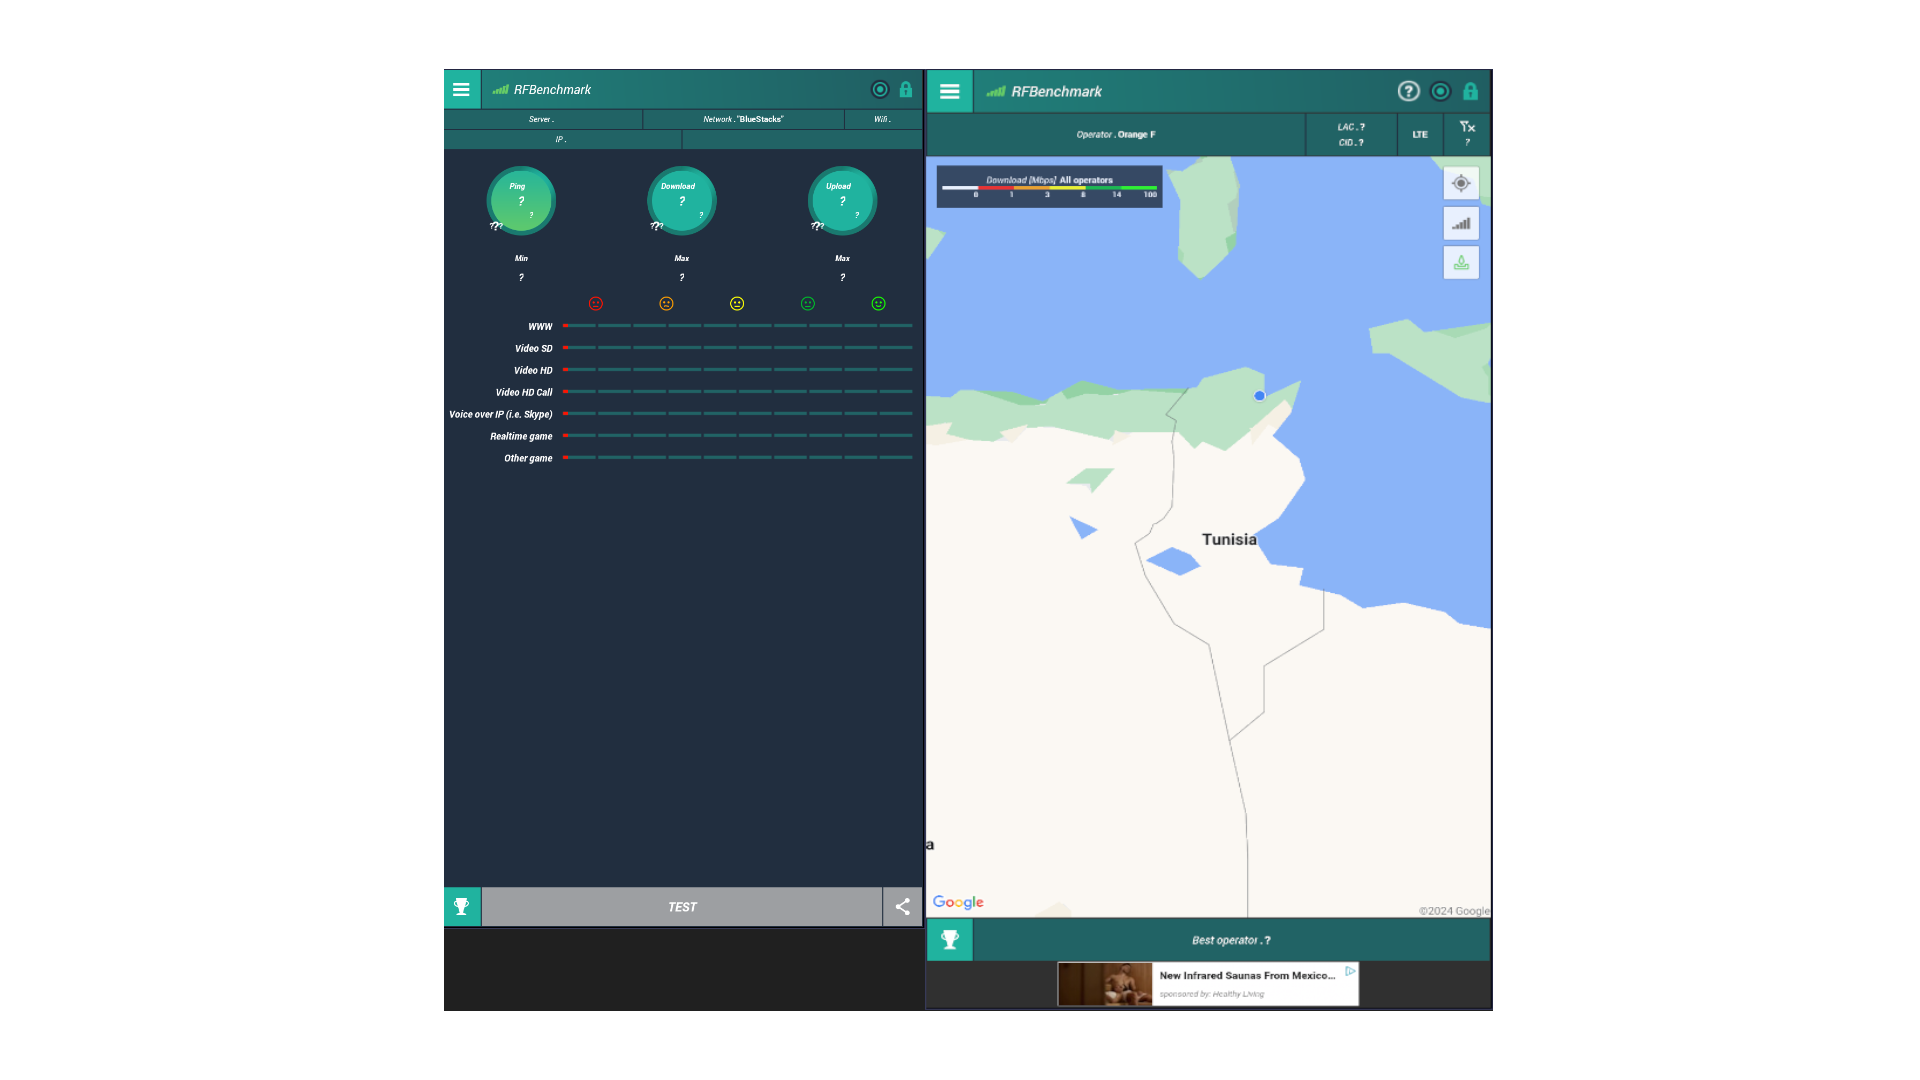
\includegraphics[height=10cm]{images/chap1/RFBenchmark.png}
    \caption{RfBenchmark demo}
    \label{fig:enter-label}
\end{figure}
\textbf{RfBenchmark} mobile app comes up with :
\begin{itemize}
    \renewcommand\labelitemi{\textbf{\Huge .}}
    \item  Speed test section
    \item Coverage map 
    \item Search functionality 
    \item Operators and networks ranking
  
\subsubsection*{Advantages}
\begin{itemize}
\renewcommand\labelitemi{\textbf{\Huge .}}
    \item Very detailed performance test
    \item User can give feedback
\end{itemize} 

\subsubsection*{Disadvantages}
\begin{itemize}
\renewcommand\labelitemi{\textbf{\Huge .}}
    \item The data is often outdated  
    \item Coverage map is not available in all counties 
    \item The data source in unknown
    \item In app adds 
    \item Complex user interface
\end{itemize} 
\end{itemize}

\section{Proposed Solution}
After planning and, in depth market research the BI4T team has introduced a new mobile app idea aimed at improving telecommunication services tracking  for individuals . This innovative concept is set to transform Quality of Service (QoS) monitoring by overcoming market challenges and providing users with options. The app is built on a foundation of both non practical needs forming the basis of its creation.
This application will let the user to :
\begin{itemize}
\renewcommand\labelitemi{\textbf{\Huge .}}
    \item Perform some tests on his network(upload and download speed and latency)  
    \item Save test's result 
    \item View  statistics and charts based on his tests
    \item View a leader-board of  best operators 
    \item View a coverage and speed map of his country
    \item Submit  feedback to the authorities and receive responses from them .
\end{itemize} 



\section{Project management Methodology}

Project management methods are essential, for carrying out projects in industries. They offer organized structures and guidelines that assist teams in planning, executing and overseeing projects from start to finish efficiently. By using these methods companies can improve project results reduce risks allocate resources better and deliver projects on time and within budget. Additionally it is important to recognize the distinctions, between project management methods to choose the appropriate approach based on project needs, team interactions and organizational goals.

\subsection{Comparative study of project management methodologies }
In the following table we'll have a comparison between widely used methods 
\begin{table}[H]
    % \centering
    % \renewcommand{\arraystretch}{2}
   
   \begin{tabular}{|p{0.15\textwidth}|p{0.20\textwidth}|p{0.13\textwidth}|p{0.14\textwidth}|p{0.25\textwidth}|p{0.1\textwidth}|}
   \hline
   
   Methodology & Core Ideas & Flexibility & Adaptability & Stakeholder Involvement & Iterative  \\ \hline

Waterfall & Sequential process with distinct phases (Requirements, Design, Implementation, Testing, Deployment). & Low & Low & Limited involvement primarily at the beginning and end of the project. & No \\ \hline

Agile & Iterative approach focusing on incremental delivery, collaboration, and flexibility. & High & High & Continuous involvement through active participation in iterations and feedback loops. & Yes \\ \hline

Scrum & Agile framework emphasizing small, cross-functional teams (Scrum Teams) working in short iterations (Sprints). & Moderate & Moderate & High involvement through roles like Product Owner, Scrum Master, and Development Team. & Yes \\ \hline

Kanban & Lean method focusing on visualizing work, limiting work in progress (WIP), and optimizing flow. & High & High & Moderate involvement, with stakeholders visualizing and managing work through Kanban boards. & Yes \\ \hline

Lean & Focuses on eliminating waste, maximizing customer value, and continuous improvement. & High & High & High involvement through value stream mapping and continuous improvement cycles. & Yes \\ \hline

\end{tabular}
    % \caption{Caption}
    % \label{tab:my_label}
     \setlength{\abovecaptionskip}{0.25cm} % Adjust the value as per your preference
    \caption{Comparison of Project Management Methodologies}
    \label{tab:Methodology_comp}
\end{table}

\subsection{SCRUM}
In our project, we have made a deliberate decision to incorporate the SCRUM methodology as our project management approach. This methodology acts as a reliable point of reference for resolving conflicts and overcoming obstacles throughout the project lifecycle. It is worth noting that SCRUM has gained high recognition and extensive adoption among successful teams in the industry.

One of the key reasons for SCRUM's popularity is the significant amount of flexibility and documentation it offers. The SCRUM framework allows us to adapt and respond to changing project requirements and priorities effectively. By breaking down the software development process into manageable sprints lasting one to four weeks, SCRUM enables us to deliver working and tested software components incrementally, ensuring that progress is continuously made.


\begin{figure}[H]
    \centering
    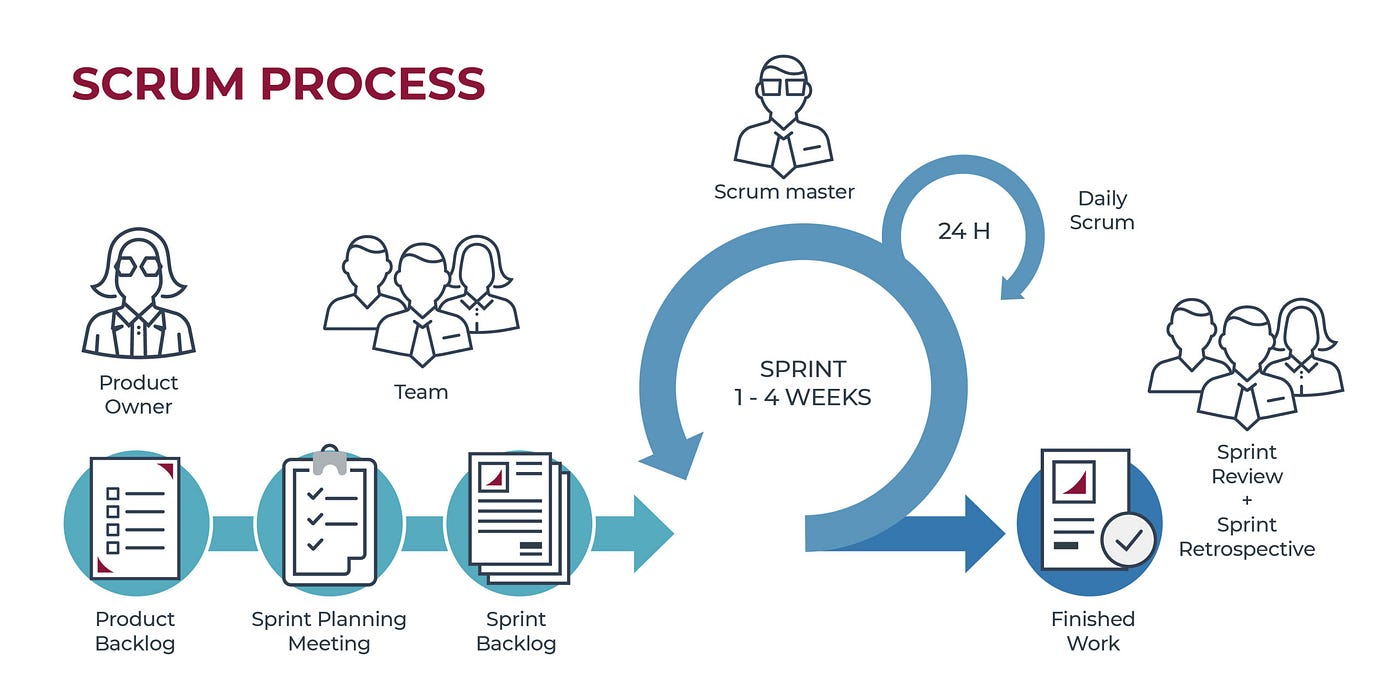
\includegraphics[height=9cm]{images/chap1/Scrum.jpg}
    \caption{Scrum Logo}
    \label{fig:enter-label}
\end{figure}

\subsection{How SCRUM works}
SCRUM follows an agile approach by breaking down project requirements into smaller, manageable chunks. This allows for iterative development and the delivery of incremental value. By treating requirements in this manner, SCRUM promotes flexibility, and accurate planning, resulting in higher client satisfaction and successful project outcomes. It allows for immediate feedback and adjustments, resulting in a higher level of client satisfaction.
This smooth workflow is attended thanks to some layers of abstraction given by SCRUM creators to separate and well define the project corner stones !

\subsection{Ceremonies}
SCRUM includes various ceremonies or meetings to facilitate collaboration and communication
\begin{itemize}
\item \textbf{Sprint Planning}: A meeting where the team determines which backlog items will be addressed in the upcoming sprint.
\item \textbf{Daily Scrum}: A brief daily meeting for the Development Team to synchronize their work, discuss progress, and identify any obstacles.
\item \textbf{Sprint Review}: A meeting at the end of each sprint where stakeholders provide feedback on the completed work and potentially adjust project priorities.
\item \textbf{Sprint Retrospective}: A reflection session where the team identifies strengths and areas for improvement in their process and teamwork for future sprints.
\end{itemize}
\subsection{Artifacts}

SCRUM also incorporates essential artifacts to have a clear version of the project state
\begin{itemize}
\item \textbf{Product Backlog}: A prioritized list of features, functionalities, and changes that need to be implemented in the project.
\item \textbf{Sprint Backlog}: A subset of items selected from the Product Backlog for a specific sprint, outlining the work to be completed.
\item \textbf{Increment}: The sum of all the completed Product Backlog items during a sprint, resulting in a potentially shippable product.
\end{itemize}

\subsection{Actors}
SCRUM involves specific actors or roles within the team to split workload and share responsibilities 
\begin{itemize}
\item \textbf{Product Owner}: The individual responsible for managing and prioritizing the Product Backlog, ensuring that the team focuses on delivering the most valuable features.
\item \textbf{Development Team}: A self-organizing group of professionals responsible for delivering the product increment during each sprint.
\item \textbf{Scrum Master}: The facilitator of the SCRUM process, ensuring that the team adheres to the framework and removing any impediments that hinder progress.
\end{itemize}
\vspace{0.5cm}
\section{Modeling language}
A modeling language serves as an standardized formal means to depict and explain systems, processes or ideas. It offers a collection of guidelines and symbols for crafting representations that illustrate the components, connections and actions, within a system or area. These languages find use across fields, like software development, system planning, data representation and business process depiction. Known examples of modeling languages encompass Unified Modeling Language (UML) Business Process Model and Notation (BPMN) Entity Relationship Diagram (ERD) and SysML (Systems Modeling Language).

\subsection{Unified modeling language (UML)}
UML is a modeling language used to depict systems in an object oriented way. It offers diagrams to illustrate behavior, interaction and structure. In class diagrams actors are depicted as classes. Entity relationship diagrams, in UML aid in simplifying database comprehension. They facilitate understanding of system elements and potential scenarios. Behavior and interaction diagrams portray behavior and message exchange. UML serves as an instrument, for representing systems designing databases and analyzing scenarios.

\begin{figure}[H]
    \centering
    
\includegraphics[height=4cm]{images/chap1/UML.png}
    \caption{Unified modeling language LOGO}
    \label{fig:enter-label}
\end{figure}

\subsection{Importance of UML}

Employing conceptual modeling during the development of information systems enables a more appropriate consideration of application needs and facilitates the abstract representation of certain aspects of physical and human systems.

\vspace{0.25cm}
\subsection*{Formal and Standardized Language}
\begin{itemize}
\renewcommand\labelitemi{\textbf{\Huge .}}
\item Ensures consistent use of UML elements for accurate representations.
\item Minimizes errors and improves development efficiency through common language.
\end{itemize}

\subsection*{Effective Communication Medium}
\begin{itemize}
\renewcommand\labelitemi{\textbf{\Huge .}}
\item Conveys complex ideas through clear visual representations.
\item Versatility and flexibility promote universal communication across teams.
\item Enables clear understanding between developers, designers, and stakeholders.
\end{itemize}

\subsection*{Tailored for Software Development}
\begin{itemize}
\renewcommand\labelitemi{\textbf{\Huge .}}
\item Designed specifically to specify, build, and document software systems.
\item Standardized notation balances design freedom with clear communication.
\item Combination of formality, standardization, communication, and modeling capabilities make UML ideal for many projects.
\item Visual diagrams offer diverse perspectives for comprehensive understanding of the software.
\end{itemize}
UML, a visual language, utilizes various diagrams. Each diagram offers a unique perspective on the software project, providing a comprehensive view of the system to be developed. These diagrams can be categorized based on whether they represent static aspects (structure) or dynamic aspects (behavior).


\begin{table}[H]
    % \centering
    % \renewcommand{\arraystretch}{2}

   \begin{tabular}{|p{0.3\textwidth}|p{0.60\textwidth}|}
   \hline
     
        \begin{center}
            \textbf{Static (structure)}
        \end{center} & 
        \begin{itemize}
            \renewcommand\labelitemi{\textbf{\Huge .}}

            \item Use cases  
            \item Classes  
            \item Components  
            \item Objects
            \item Deployment

        \end{itemize}  \\   \hline

        
        \begin{center}
            \textbf{Dynamic (behavioral)}
        \end{center} & 
        \begin{itemize}
            \renewcommand\labelitemi{\textbf{\Huge .}}
            
            \item  Sequences  
            \item  Activity  
            \item  State-transition  
            \item  Cooperation

        \end{itemize}
        \\   \hline

        
\end{tabular}
    \caption{UML Static \& Dynamic Diagrams }
    \label{tab:UML_diagrams_list}
     \setlength{\abovecaptionskip}{0.25cm}
\end{table}

In this project, we make use of two types of UML diagrams:

\vspace{0.25cm}

\begin{itemize}
\renewcommand\labelitemi{\textbf{\Huge .}}
\item Use case diagrams: These diagrams outline the functions of the application from the user's point of view.
\item Sequence diagrams: These diagrams illustrate the chronological and behavioral interactions between objects within the system.
\item Class diagrams: These diagrams depict the static structure of a system, including the classes, their attributes, methods, and the relationships between them.
\end{itemize}

\vspace{0.25cm}

\section{Terminologies}
As we delve into the project, it's helpful to clarify some important terminologies
\subsection{Business Intelligence}
Business intelligence combines business analytics, data mining, data visualization, data tools and infrastructure, and best practices to help organizations make more data-driven decisions. In practice, you know you’ve got modern business intelligence when you have a comprehensive view of your organization’s data and use that data to drive change, eliminate inefficiencies, and quickly adapt to market or supply changes. Modern BI solutions prioritize flexible self-service analysis, governed data on trusted platforms, empowered business users, and speed to insight
% \cite{https://www.tableau.com/learn/articles/business-intelligence}

\begin{figure}[H]
    \centering
    
\includegraphics[height=6cm]{images/chap1/BI.jpeg}
    \caption{BI illustration}
    \label{fig:enter-label}
\end{figure}
\subsection*{Key Performance Indicators}
Key Performance Indicators (KPIs) are the critical (key) quantifiable indicators of progress toward an intended result. KPIs provide a focus for strategic and operational improvement, create an analytical basis for decision making and help focus attention on what matters most.

Managing with the use of KPIs includes setting targets (the desired level of performance) and tracking progress against those targets.

Managing with KPIs often means working to improve performance using leading indicators, which are precursors of future success, that will later drive desired impacts indicated with lagging measures.
% \cite{https://www.kpi.org/kpi-basics/}
\subsection{Mobile Development}
Mobile application development is the process of creating software applications that run on a mobile device, and a typical mobile application utilizes a network connection to work with remote computing resources. Hence, the mobile development process involves creating installable software bundles (code, binaries, assets, etc.) , implementing backend services such as data access with an API, and testing the application on target devices.
% \cite{https://aws.amazon.com/mobile/mobile-application-development/#:~:text=Mobile%20application%20development%20is%20the,work%20with%20remote%20computing%20resources.}
\subsection*{Native Development}
Native app development means creating a mobile application that is tailored and dedicated to a specified platform like iOS, or Android. 

Because native applications are built specifically for the operating system, they provide higher user engagement than hybrid apps. Native mobile apps generally perform and look better than their web-based counterparts, which must serve numerous platforms. Furthermore, native mobile applications have access to devise hardware and capabilities, such as sensors and cameras, that are not available via a mobile browser interface alone.
% \cite{https://mdevelopers.com/blog/what-is-a-native-mobile-app-development-}
The two main modern native languages used in the industry are Swift for IOS apps and Kotlin for Android .
\begin{figure}[H]
    \centering
    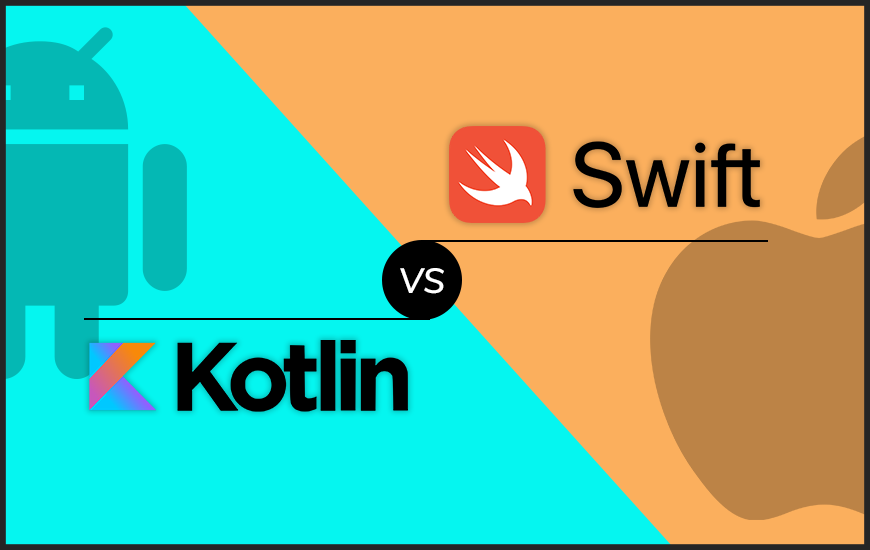
\includegraphics[height=6cm]{images/chap1/kotlin_swift.png}
    \caption{Kotlin\&Swift Logo}
    \label{fig:enter-label}
\end{figure}
\subsection*{Hybrid Development}
You create a hybrid or cross-platform mobile applications from a single codebase. The goal of cross-platform app development is to target different operating systems with one project. You create these apps using cross-platform frameworks, which use platform-specific SDKs (Android SDKs and iOS SDKs) from a unified API. This enables you to easily access the different platform SDKs and libraries.

Private companies create these frameworks. Examples of popular cross-platform frameworks include:

\begin{itemize}
\renewcommand\labelitemi{\textbf{\Huge .}}
\item React Native by Meta. It uses JavaScript as the programming language.
\item Flutter by Google. It uses Dart as the programming language.
\end{itemize}
\begin{figure}[H]
    \centering
    
\includegraphics[height=6cm]{images/chap1/reactNative_Flutter.png}
    \caption{Kotlin\&Swift Logo}
    \label{fig:enter-label}
\end{figure}
\subsection*{The benefit of hybrid application}
% \usepackage{tabularray}
\begin{longtblr}[
  \caption = {Native vs Cross-platform App Developement}
]{
  width = \linewidth,
  colspec = {Q[163]Q[319]Q[460]},
  cells = {c},
  hlines,
  vlines,
}
Feature                     & Cross-Platform App Development                                & Native App Development                                                                      \\
Development Time            & Faster development due to a single codebase                   & Slower development as separate codebases are needed for each platform (Android  iOS)        \\
Development Cost            & Generally lower cost due to code reusability                  & Generally higher cost due to needing separate development teams or expertise                \\
Performance                 & May have slightly slower performance due to abstraction layer & Offers optimal performance as code is tailored to the specific platform                     \\
User Experience (UX)        & May have a less native look and feel                          & Provides a platform-specific UX that feels natural to users                                 \\
Access to Platform Features & May have limitations in accessing all native features         & Full access to all platform features and functionalities                                    \\
Maintenance                 & Easier to maintain due to a single codebase                   & More complex to maintain as separate codebases need updates                                 \\
Learning Curve              & Requires knowledge of cross-platform frameworks               & Requires knowledge of platform-specific languages (e.g., Swift for iOS, Kotlin for Android) \\
Market Reach                & Reaches a wider audience with a single app                    & Reaches platform-specific audiences with separate apps                                      
\end{longtblr}




\vspace{0.5cm}



\section*{Conclusion}
In summary this chapter has given an overview of the internship framework and the organization hosting it. It has defined the projects scope provided examples, from the market explained the project management method chosen talked about the language and software tools used and clarified terms. This examination has laid a groundwork for chapters preparing us for a thorough analysis and implementation of the project. With an understanding of the context project boundaries, methodology employed and necessary tools we are ready to move into the execution phase, with clarity and purpose.




% \titleformat{\chapter}[block]
% {\filcenter\bfseries\Huge}
% {\xrfill[0.4ex]{5pt}\ \thechapter.\ \xrfill[0.4ex]{5pt}}
% {0pt}
% {\xrfill[0.4ex]{5pt}\ \MakeUppercase{#1}\ \xrfill[0.4ex]{5pt}}

\chapter*{Chapter 2}

\markboth{Chapter 2:Planning \& Specification of requirements}{Planning \& Specification of requirements} %pour afficher l'entete
\addcontentsline{toc}{chapter}{2  Planning \& Specification of requirements}





\etocsettocstyle{\subsection*{Plan}}{}
\vspace{0.25cm}

\setcounter{tocdepth}{1}
\headrule{
\vspace{0.5cm}

\begin{center}
    \textsc{\textbf {\Huge Planning \& Specification of requirements}} 
\end{center}
}
\headrule


\localtableofcontents
\newpage


\setcounter{chapter}{2}
\setcounter{section}{0}
\setcounter{table}{0} % Reset the table counter to 0
\setcounter{figure}{0} 


\section*{Introduction}

In this chapter, we will start by analyzing and specifying the requirements of our application, explaining its functional and non-functional requirements. Next, we will present the overall use case diagram, specifying the different actors. Finally, we will detail the project management using the Scrum methodology, presenting the architecture adopted for our application.



\section{Requirement specification}
Requirement specification, also known as documentation, is a process of jotting down all the system and user requirements in the form of a document. These requirements must be clear, complete, comprehensive, and consistent. \cite{VISURE}
% \cite{"https://visuresolutions.com/blog/requirements-specification/#:~:text=Requirement%20specification%2C%20also%20known%20as,complete%2C%20comprehensive%2C%20and%20consistent."}
\subsection{Functional requirements }
The functional requirements, as their name implies outline the operations of the system to be developed. They detail what the system will entail and how it will operate to meet user requirements. These requirements offer an account of how the system should react to instructions, its capabilities and user expectations. 
For our application these are the functional requirements for every kind of user: \newline
\textbf{For a guest }
\begin{itemize}
\renewcommand\labelitemi{\textbf{\Huge .}}
    \item Create an account 
    \item Test his network
\end{itemize} 
\textbf{For a registered user :}
\begin{itemize}
\renewcommand\labelitemi{\textbf{\Huge .}}
    \item Login to his account  
    \item Manage his account  
    \item Test his network 
    \item View previous results  
    \item Save test result 
    \item View  statistics and charts based on his tests
    \item View a leader-board  
    \item View a coverage and speed map of his country
    \item Submit  feedback.
\end{itemize} 
\subsection{Non-functional requirements }
The applications non functional requirements cover both the goals related to system performance and environmental limitations usually expressed as targets that the system needs to achieve. These guidelines outline the limits and constraints, during development to ensure they do not affect the functionality of the application. Additionally non functional requirements are essential for staying in sync with requirements and promoting qualities, like cost effectiveness user friendliness and ease of access. 
\begin{itemize}
\renewcommand\labelitemi{\textbf{\Huge .}}
\item \textbf{Simplicity:} The application boasts user-friendly interfaces, ensuring ease of use for all users.
\item \textbf{Performance:} The application efficiently meets all user requirements in an optimal manner.
\item \textbf{Security:} Ensuring robust security measures, access to information is restricted to authorized users via unique usernames and passwords.

\item \textbf{Extensibility:} The application is designed with extensibility in mind, allowing for future updates and enhancements.
\item \textbf{Ergonomics:} The chosen color scheme prioritizes user comfort, promoting ease of use and reducing strain on the eyes.
\end{itemize}

\section{Identification and structuring of use cases}

\subsection{Actors:}
UML defines an actors as every external entity of the system and has a role played within this system ,an actor can have multiple forms like human, an electronic device or in some cases an other system .
Our application will be mainly used by two actors as described below :


\begin{table}[H]
    % \centering
    % \renewcommand{\arraystretch}{2}

  
   \begin{tabular}{|p{0.18\textwidth}|p{0.75\textwidth}|}
   \hline
     
        \begin{center}
            \textbf{Guest User}
        \end{center} & 
        \begin{itemize}
            \renewcommand\labelitemi{\textbf{\Huge .}}

            \item Test his network
            \item Create an account

        \end{itemize}  \\   \hline
        \begin{center}
            \textbf{User}
        \end{center} & 
        \begin{itemize}
            \renewcommand\labelitemi{\textbf{\Huge .}}

            \item Authenticate to the app
            \item Test his network
            \item View Reports
            \item Consult Map
            \item Consult Leader-board
            \item Submit feedback 

        \end{itemize}  \\   \hline



        
\end{tabular}
     \caption{Actors Table}
    \label{tab:my_label}
     \setlength{\abovecaptionskip}{0.25cm}
\end{table}

\newpage 

\subsection{General use case diagram : }

The use case diagram outlines the functions of the application from the user's point of view.This diagram will cover the global use cases of our application.


\begin{figure}[H]
    \centering
    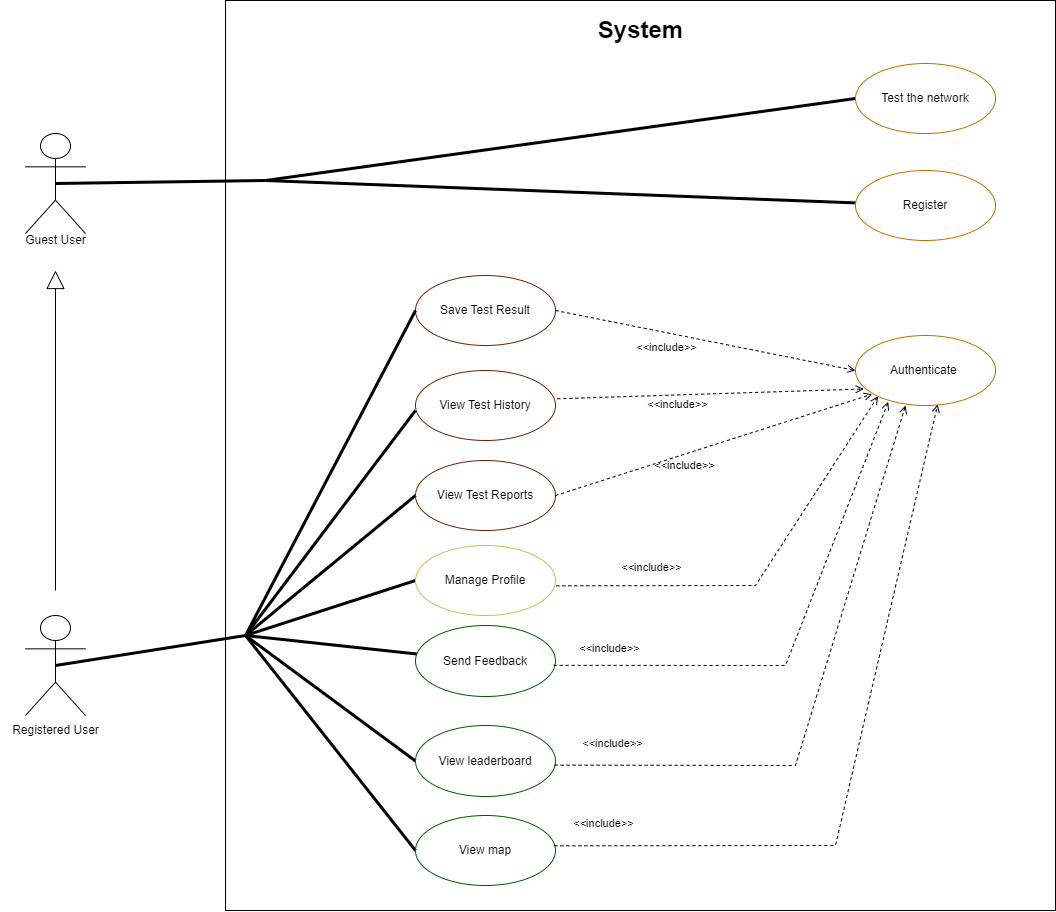
\includegraphics[width=1\textwidth]{images/chap1/gloabalUC.png}
    \caption{Global Use Case Diagram}
    \label{fig:enter-label}
\end{figure}

\newpage

\subsection{General class diagram : }

The class diagram provides a visual representation ofthe static structure of a system, including the classes, their attributes, methods, and the relationships between them.This diagram will cover the global class diagram of our application.
% Not done yet
\begin{figure}[H]
    \centering
    \includegraphics[width=0.97\textwidth]{images/global-class.pngp}
    \caption{General class diagram - Not done yet}
    \label{fig:enter-label}
\end{figure}




\newpage

\section{Project management with Scrum}

\subsection{Scrum projection on our project}
By adopting SCRUM as a project management approach we need to define actors 
and provide a product backlog from specified requirements earlier 
\subsubsection{Scrum actors in our team}

\begin{table}[H]
    \centering
    \begin{tabular}{|p{5cm}|p{5cm}|p{6.5cm}|}
    \hline
    \textbf{Member} & \textbf{Role} & \textbf{Task} \\ \hline
    \begin{center}
        \textbf{Bilel Othmen}
    \end{center} & \begin{itemize}
        \item Product Owner
    \end{itemize} & \begin{itemize}
        \item Identification of requirements and functionalities to be implemented
    \end{itemize} \\ \hline

    \begin{center}
        \textbf{Nizar Ben Soltane}
    \end{center} & \begin{itemize}
        \item Scrum Master
    \end{itemize} & \begin{itemize}
        \item Project Validation
    \end{itemize} \\ \hline

    \begin{center}
        \textbf{Hammami Mohamed Yacin}
    \end{center} & \begin{itemize}
        \item Development Team
    \end{itemize} & \begin{itemize}
        \item Development
        \item Validation and Testing
        \item Deployment
    \end{itemize} \\ \hline
    \end{tabular}
    \caption{SCRUM Actors}
    \label{tab:my_label}
    \setlength{\abovecaptionskip}{0.25cm}
\end{table}

\newpage


\subsection{Product Backlog}
From the requirements specified  earlier and the global use case diagram , we can extract a product backlog to be our guide in through this project 


\begin{table}[H]
% \begin{tabular}{|p{5cm}|p{5cm}|p{6.5cm}|}
\begin{tabular}{|p{0.5cm}|p{3cm}|p{7cm}|p{2cm}|p{2cm}|}
\hline
ID & Epic           & Description                                                               & Priority & Complexity \\ \hline
1  & Configuration & Administrator can specify the desired parameter that  the application will work with  & High     & basic      \\ \hline
2  & Authentication & User can authenticate to the app through a robust authentication system   & High     & basic      \\ \hline
3  & Network Test     & User can test his network, see results and save them                      & High     & medium     \\ \hline
4  & Cartography    & User can inspect the network state in his country in specific time period & High     & High       \\ \hline
5  & Reporting      & User can see detailed reports based on his tests                          & medium   & medium     \\ \hline
6  & Feedback       & User can send feedback or report issues to authorities                    & Low      & basic      \\ \hline
\end{tabular}
\caption{Product Backlog}
\label{tab:backlog}
\end{table}


\newpage

\section{Sprint Planning}

The 2.4 table illustrates the distribution of sprints and the duration of each one

\begin{table}[H]
    % \centering
    \renewcommand{\arraystretch}{1.5}
   
   \begin{tabular}{|p{0.15\textwidth}|p{0.61\textwidth}|p{0.15\textwidth}|}
   \hline
   \centering
   \textbf{Sprints } &  \textbf{Sprint Functionality} &\textbf{Duration}
\\ \hline
        \centering
       \textbf{Sprint 1}  &  
       \begin{itemize}[left=0pt,label={\textbf{-}}]
           \item Configurable application
           \item Navigation system
           \item Authentication system
       \end{itemize}
       & 
       \begin{itemize}[left=0pt,label={\textbf{-}}]
           \item  5 days
           \item  5 days
           \item  10 days
       \end{itemize}
       \\ \hline

       \centering
       \textbf{Sprint 2}  &  
       \begin{itemize}[left=0pt,label={\textbf{-}}]
           \item Map
           \item Leader-board 
       \end{itemize}
       &  \begin{itemize}[left=0pt,label={\textbf{-}}]
           \item  15 days
           \item  15 days
        
       \end{itemize} \\ \hline
       \centering
       \textbf{Sprint 3}  &  
       \begin{itemize}[left=0pt,label={\textbf{-}}]
           \item Network testing
           \item Report generation
       \end{itemize}
       &  \begin{itemize}[left=0pt,label={\textbf{-}}]
           \item  15 days
           \item  15 days
        
       \end{itemize} \\ \hline
       \centering
       \textbf{Sprint 4}  &  
       \begin{itemize}[left=0pt,label={\textbf{-}}]
           \item Feedback and reviews
       \end{itemize}
       &  \begin{itemize}[left=0pt,label={\textbf{-}}]
           \item  10 days
       \end{itemize} \\ \hline

       
       
\end{tabular}
     \caption{Sprint Planning Table}
    \label{tab:my_label}
     \setlength{\abovecaptionskip}{0.25cm}
\end{table}


\section{Working environment}

In this section, we provide details about the hardware and software environments that have been provided for our project.


\subsection{Hardware environment }
The technical specifications of the devices used are listed in the following table : 
\vspace{0.25cm}
\newpage
\begin{large}
    \textbf{Computer specifications}
\end{large}
\vspace{0.25cm}

\begin{table}[H]
    % \centering
    \renewcommand{\arraystretch}{1.5}
   \begin{tabular}{|p{0.3\textwidth}|p{0.61\textwidth}|}
   \hline
    
       \textbf{Computer} & Lenovo IdeaPad3 \\ \hline
       \textbf{Processor} & i5-10210U  \\ \hline
       \textbf{RAM} & 20 \\ \hline
       \textbf{Hard disk} & 512 SSD \\ \hline
       \textbf{Graphic card} & MX130  \\ \hline
       \textbf{Operating System} &Windows 10 Pro \\ \hline

\end{tabular}
     \caption{Computer specifications Table}
    \label{tab:my_label}
    % \setlength{\abovecaptionskip}{0.25cm}
\end{table}

\begin{large}
    \textbf{Smartphones specifications}
\end{large}

\begin{table}[H]
    % \centering
    \renewcommand{\arraystretch}{1.5}
    \setlength{\belowcaptionskip}{0.25cm}
    

   \begin{tabular}{|p{0.3\textwidth}|p{0.61\textwidth}|}
   \hline
    
       \textbf{Model name} & Samsung Galaxy A04 \\ \hline
       \textbf{OS} & Android 13\\ \hline
       \textbf{RAM} & 4 Gb \\ \hline
       \textbf{Battery} &  5000 mAh \\ \hline
       \textbf{Storage} & 64 Gb \\ \hline

\end{tabular}
   
    % \setlength{\abovecaptionskip}{0.25cm}
    \caption{Smartphones specifications Table}
    \label{tab:my_label}
\end{table}

\section{Software kit}
In recognition of its importance to the project's accomplishment, we'll be specifying the software  kit  used in this journey.  This information will also be helpful for anyone with questions about the project's technology stack.
\subsection{Project Management}
\subsection*{Jira}
For tracking our project and letting all team members to  have an updated vision on its progress we used Jira as Project management tool .
Jira Software is the \#1 agile project management tool used by teams to plan, track, release and support world-class software with confidence. It is the single source of truth for your entire development lifecycle, empowering autonomous teams with the context to move quickly while staying connected to the greater business goal. Whether used to manage simple projects or to power your DevOps practices, Jira Software makes it easy for teams to move work forward, stay aligned, and communicate in context.\cite{Jira}
% \cite{https://www.atlassian.com/software/jira/guides/getting-started/introduction}
\begin{figure}[H]
    \centering
    
\includegraphics[height=4cm]{images/chap1/jira.png}
    \caption{Jira Logo}
    \label{fig:enter-label}
\end{figure}
\subsection{Version Controle}
\subsection*{GitLab}
We used GitLab to store our application code and to facilitate integration in a CI/CD pipeline .
GitLab is an Open Source code repository and collaborative software development platform for large DevOps and DevSecOps projects. GitLab is free for individuals.

GitLab offers a location for online code storage and capabilities for issue tracking and CI/CD. The repository enables hosting different development chains and versions.\cite{GitLab}
% \cite{https://www.techtarget.com/whatis/definition/GitLab}
\begin{figure}[H]
    \centering
    
\includegraphics[height=4cm]{images/chap1/gitlab.png}
    \caption{GitLab Logo}
    \label{fig:enter-label}
\end{figure}

\subsection{Modeling}
\subsection*{Drawio}
We used Drawio to draw all diagrams used in this report,
draw.io is a technology stack for building diagramming applications, and the world’s most widely used browser-based end-user diagramming software. \cite{Drawio}
% \cite{https://www.drawio.com/about}
\begin{figure}[H]
    \centering
    
\includegraphics[height=4cm]{images/chap1/drawio.png}
    \caption{Drawio Logo}
    \label{fig:enter-label}
\end{figure}
% \subsection{Report Writing}
% \subsection*{LaTex}
% LaTeX is widely used in academia for the communication and publication of scientific documents and technical note-taking in many fields. It also has a prominent role in the preparation and publication of books and articles that contain complex multilingual materials, such as Arabic and Greek.LaTeX uses the TeX typesetting program for formatting its output, and is itself written in the TeX macro language.
% % \cite{https://en.wikipedia.org/wiki/LaTeX}
% \begin{figure}[H]
%     \centering
%     
\includegraphics[height=4cm]{images/chap1/Latex-logo.png}
%     \caption{LaTex Logo}
%     \label{fig:enter-label}
% \end{figure}
% \subsection*{Overleaf}
% Overleaf’s market-leading collaboration technology is now in use by over 15 million researchers, students, and teachers in institutions, labs, and industry worldwide.
% % \cite{https://www.overleaf.com/about}
% \begin{figure}[H]
%     \centering
%     
\includegraphics[height=4cm]{images/chap1/overleaf_wide_colour_light_bg.png}
%     \caption{Overleaf Logo}
%     \label{fig:enter-label}
% \end{figure}
\subsection{Development}
\subsubsection{Programming Language and Database}
\subsubsection*{Spring Boot}
As a robust backend we chose springboot as backend framework .
Java Spring Boot is an open-source tool that makes it easier to use Java-based frameworks to create microservices and web apps.\cite{Springboot} 
% \cite{https://azure.microsoft.com/en-us/resources/cloud-computing-dictionary/what-is-java-spring-boot}
\begin{figure}[H]
    \centering
    
\includegraphics[height=6cm]{images/chap1/springJava.png}
    \caption{Springboot \& Java Logo}
    \label{fig:enter-label}
\end{figure}
\subsubsection*{React Native}
To have a modern and complex UI , and to have a cross platform application , we adopted React-Native, 
React Native is an open-source UI software framework created by Meta Platforms, Inc. It is used to develop applications for Android: Android TV,iOS:, macOS, tvOS,Web, Windows and UWP by enabling developers to use the React framework along with native platform capabilities.\cite{ReactNative}
% \cite{https://en.wikipedia.org/wiki/React_Native}
\begin{figure}[H]
    \centering
    
\includegraphics[height=6cm]{images/chap1/reactnativeJS.png}
    \caption{React native \& Javascript Logo}
    \label{fig:enter-label}
\end{figure}
\subsubsection*{Expo}
To have a better developer experience building this application , we used Expo to benefit its outstanding features .
Expo is a set of tools and services built around React Native and, while it has many features, the most relevant feature for us right now is that it can get you writing a React Native app within minutes. You will only need a recent version of Node.js and a phone or emulator. \cite{Expo}
% \cite{https://reactnative.dev/docs/environment-setup#:~:text=Expo%20is%20a%20set%20of,and%20a%20phone%20or%20emulator.}
\begin{figure}[H]
    \centering
    
\includegraphics[height=6cm]{images/chap1/expo.png}
    \caption{Expo Logo}
    \label{fig:enter-label}
\end{figure}

\subsubsection*{PostgreSQL}
To store all application's data , our decision was PostgreSQL as a RDBMS. 
PostgreSQL is an advanced, enterprise-class, and open-source relational database system. PostgreSQL supports both SQL (relational) and JSON (non-relational) querying.\cite{PostgreSQL}
% \cite{https://www.postgresqltutorial.com/postgresql-getting-started/what-is-postgresql/}
\begin{figure}[H]
    \centering
    
\includegraphics[height=4cm]{images/chap1/postgres.png}
    \caption{PostgreSQL Logo}
    \label{fig:enter-label}
\end{figure}



\subsection{Code Editor}
\subsubsection*{VsCode}
To write code , test it and push it to GitLab ,VsCode was a great tool for providing that and more features to facilitate the development journey .
Visual Studio Code is a free coding editor that helps you start coding quickly. Use it to code in any programming language, without switching editors. Visual Studio Code has support for many languages.\cite{VSCode}
% \cite{https://code.visualstudio.com/learn}
\begin{figure}[H]
    \centering
    
\includegraphics[height=4cm]{images/chap1/vscode.jpg}
    \caption{Vscode Logo}
    \label{fig:enter-label}
\end{figure}
\subsection{Testing}
\subsubsection*{Postman}
To test our API endpoints , we used Postman .
Postman is an API platform for building and using APIs. Postman simplifies each step of the API lifecycle and streamlines collaboration so you can create better APIs—faster.\cite{Postman}
% \cite{https://www.postman.com/product/what-is-postman/}
\begin{figure}[H]
    \centering
    
\includegraphics[height=4cm]{images/chap1/postman.jpg}
    \caption{Postman Logo}
    \label{fig:enter-label}
\end{figure}





\subsection{Application's Architecture}
The structure of an application, known as application architecture encompasses its core design elements, including components, their connections and the guiding design principles. It covers aspects such, as;
\begin{enumerate}
    \item  \underline{\textbf{Component Arrangement}:}
 This involves identifying the parts or sections of the application. How they interact with each other. Components can range from user interfaces to databases, services, APIs and external systems.

\item  \underline{\textbf{Data Handling}:} How information is stored, retrieved, updated and managed within the application. This includes selecting databases, data models and storage methods.

\item  \underline{\textbf{Communication Methods}:} Specifies how different components communicate with each other. This could involve asynchronous communication using protocols, like HTTP, WebSockets or message queues.

\item  \underline{Handling Concurrency and Scalability:} How the application manages users concurrently. Expands to handle increased loads. Considerations include managing threads load distribution strategies and horizontal expansion.
\end{enumerate}
\subsubsection{MVC Architecture}
In this project we adopted the Model-View-Controller Architecture known as MVC ,to have an enhanced code organization, and to facilitate maintenance and scalability , in fact separate the application's logic into distinct layers, each of which holds a specific set of tasks as follow :
\begin{itemize}
    \item \textbf{Model:} The layer that manages the applications data operations is responsible, for tasks like storing and retrieving data from databases. It also includes features for validating data and performing data related functions. Its main role is to maintain the integrity and accessibility of all data aspects.

    \item \textbf{View: }The layer that showcases the user interface needed for interacting with the application consists of components for displaying data and enabling user interaction. This may include elements such as buttons, links, tables, dropdown menus or input fields.

    \item \textbf{Controller: }The layer that coordinates the applications logic facilitates communication, between the view and model layers. Regarded as the engine of the application it oversees the flow and synchronization of operations.

\end{itemize}
\begin{figure}[H]
    \centering
    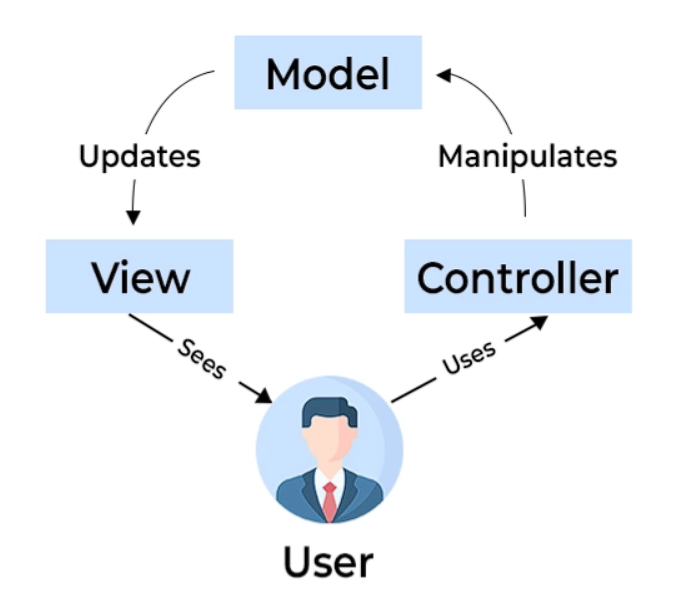
\includegraphics[height=7cm]{images/chap1/mvc.png}
    \caption{MVC architecture}
    \label{fig:enter-label}
\end{figure}






\section*{Conclusion}

During this chapter, we identified the functional and non-functional requirements of the system, as well as the main actors and their roles. Afterwards, we identified the product backlog and sprint planning. We concluded the chapter by explaining the architecture of our application. In the next chapter, we will begin the development of Sprint 1.


% \titleformat{\chapter}[block]
% {\filcenter\bfseries\Huge}
% {\xrfill[0.4ex]{5pt}\ \thechapter.\ \xrfill[0.4ex]{5pt}}
% {0pt}
% {\xrfill[0.4ex]{5pt}\ \MakeUppercase{#1}\ \xrfill[0.4ex]{5pt}}

\chapter*{Chapter 3}

\markboth{Sprint 1 : Application Skeleton }{3 Sprint 1 : Application Skeleton} %pour afficher l'entete
 \addcontentsline{toc}{chapter}{3 Sprint 1 : Application Skeleton}



\setcounter{chapter}{3}
\setcounter{section}{0}
\setcounter{table}{0} 
\setcounter{figure}{0} 


\etocsettocstyle{\subsection*{Plan}}{}
\vspace{0.25cm}

\setcounter{tocdepth}{1}
\headrule{
\vspace{0.5cm}

\begin{center}
    \textsc{\textbf {\Huge Sprint 1 : Application Skeleton}} 
\end{center}
}
\headrule


\localtableofcontents
\newpage






\section*{Introduction}
After having a good understanding of the project scope and requirements in the previous chapter.
In this chapter, we will tackle the realisation of  the first sprint of our project which handles the development of the core functionalities of the application like configuration,navigation and authentication . We will cover the planning and analysis of this sprint also we will go through the  implementation and testing and finally showcasing the artifacts .

\section{Sprint 1 Backlog}
The sprint backlog is a detailed list of tasks and user stories selected for completion within the current sprint, guiding the development team's work towards achieving the sprint goal. It serves as a dynamic, prioritized plan that evolves as the team progresses and new information emerges.
The table below describes the backlog of the firs sprint :



\begin{table}[H]
    % \centering
    \renewcommand{\arraystretch}{1.2}
    \setlength{\belowcaptionskip}{0.25cm}
 
   \begin{tabular}{|p{0.05\textwidth}|p{0.25\textwidth}|p{0.29\textwidth}|p{0.34\textwidth}|}
   \hline
   \textbf{ID}  &  \textbf{User Story } & \textbf{Description} & \textbf{Task} \\ \hline


   
   \begin{center}
       \textbf{1}
   \end{center} & \begin{center}
       As an administrator , I can enter my parameters to  configure the application 
   \end{center} &
   The administrator is capable to define the modules , access level and the constants used all over the application 
   & 

       \begin{itemize}[left=0pt, label={\textbf{\Huge .}}]
       % \renewcommand\labelitemi{\textbf{\Huge .}}
            \item Develop Constants service   
            \item Develop Modules service   
            \item Develop Init  service   

        \end{itemize} \\ \hline


   \begin{center}
       \textbf{2}
   \end{center} & \begin{center}
       As a  user, I want to navigate through the application modules 
   \end{center} &
   
  The  user can navigate between screens and interact with the application's modules  & 

       \begin{itemize}[left=0pt, label={\textbf{\Huge .}}]
            \item Develop a drawer navigator 
            \item Develop a tabs navigator
            \item Develop modules screens

        \end{itemize} \\ \hline
        % &&&&&&&&&&&&&&&&&&&&&&&&
   \begin{center}
       \textbf{3}
   \end{center} & \begin{center}
       As a  user, I want to authenticate to the application and access protected modules
   \end{center} &
   
  The  user can create an account , sign in to the app in order to access restricted modules,also he can reset his password  & 

       \begin{itemize}[left=0pt, label={\textbf{\Huge .}}]
            \item Develop application with navigation and protected pages
            \item Develop login interface
            \item Develop register interface
            \item Develop forget password interface
            \item Develop authentication backend
        \end{itemize} \\ \hline
\begin{center}
       \textbf{4}
\end{center} & \begin{center}
       As a registered user, I want to edit my account information
   \end{center} &Registered users can update their credentials such as name, phone number, password 
   &
   \begin{itemize}[left=0pt, label={\textbf{\Huge .}}]
            \item Develop user profile interface
            \item Implement the backend for managing user account 
            \end{itemize} \\ \hline
\end{tabular}
       \caption{Sprint 1 Backlog}
        \label{tab:my_label}
    
\end{table}
\section{Sprint 1 use case diagram}
From the user stories mentioned earlier we can define a use case diagram for this sprint.
\begin{figure}[H] 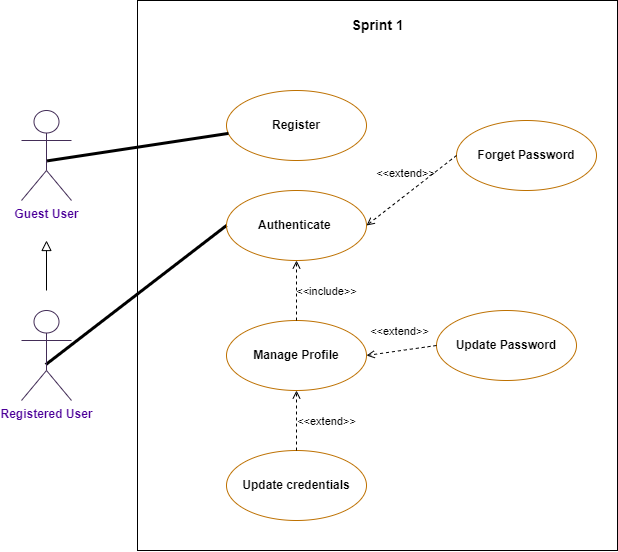
\includegraphics[height=12cm]{images/chap2/Sprint1UC.png}
    \caption{Sprint 1 use case diagram}
    \label{fig:enter-label}
\end{figure}


\section{User story n°1 : Configurable application}
Since this application is meant to be purchased by many clients , we provided the luxury of customization and to grant for every client the possibility of having an application that meets his needs .
This is done thanks to the services that import the clients on starting the application ,this process can be better described with the next illustration :

\begin{figure}[H] 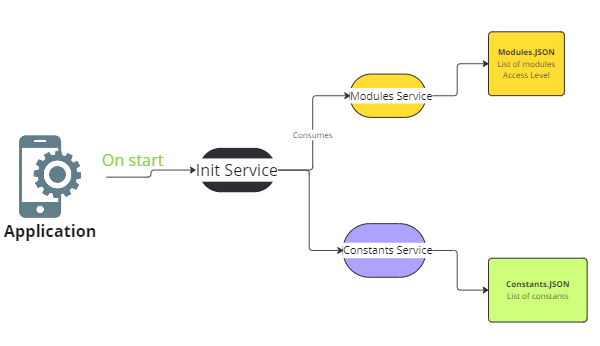
\includegraphics[width=0.90\textwidth]{images/chap2/config.png}
    \caption{Configurable Application illustration}
    \label{fig:enter-label}
\end{figure}

This approach is based on consuming raw values from JSON files that the application's owner can edit manually or via an interface in our case we split the load of data on specific services to ensure the ease of use  and the possibility for scaling 



\section{User story n°2 : Navigation}
As the global use case diagram shows that the application has some modules that require authentication whereas others don't ,so we developed a mechanism to attend this behavior , the following flowchart explain it well
\begin{figure}[H] 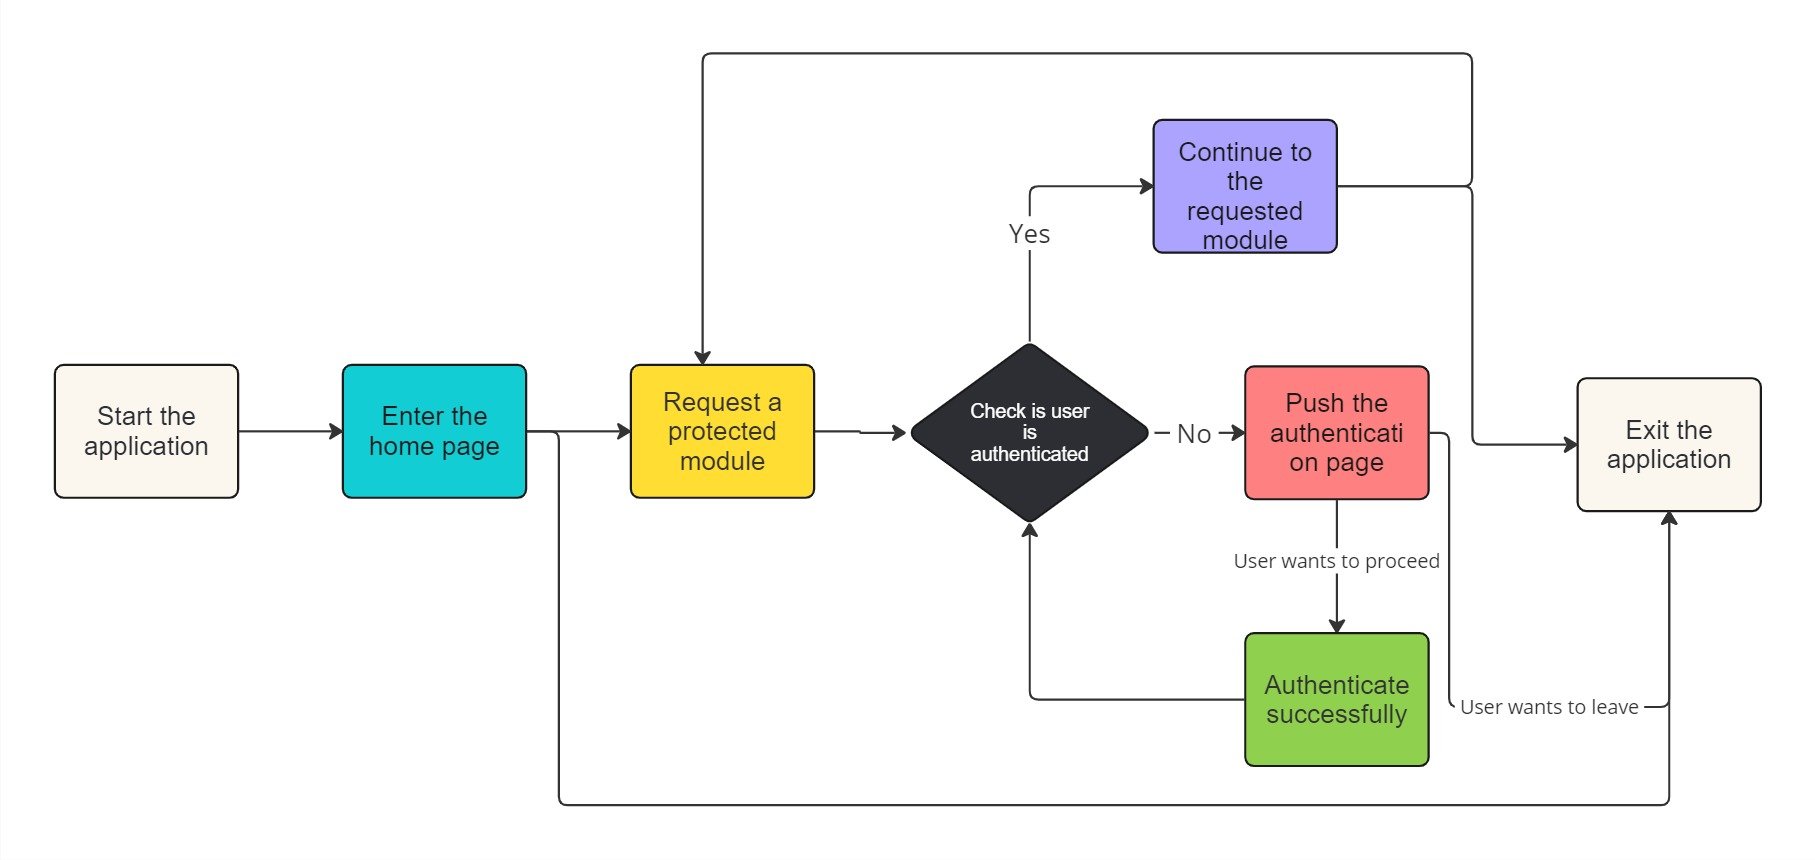
\includegraphics[height=8cm]{images/chap2/Pmdl.jpg}
    \caption{Module protection flowchart}
    \label{fig:enter-label}
\end{figure}
\newpage
\subsection{Realization}
The navigation system is split to two main parts: module navigator with bottom tabs and the application management with the drawer navigator
\begin{figure}[H]
\begin{minipage}{0.3\textwidth}
    \centering
    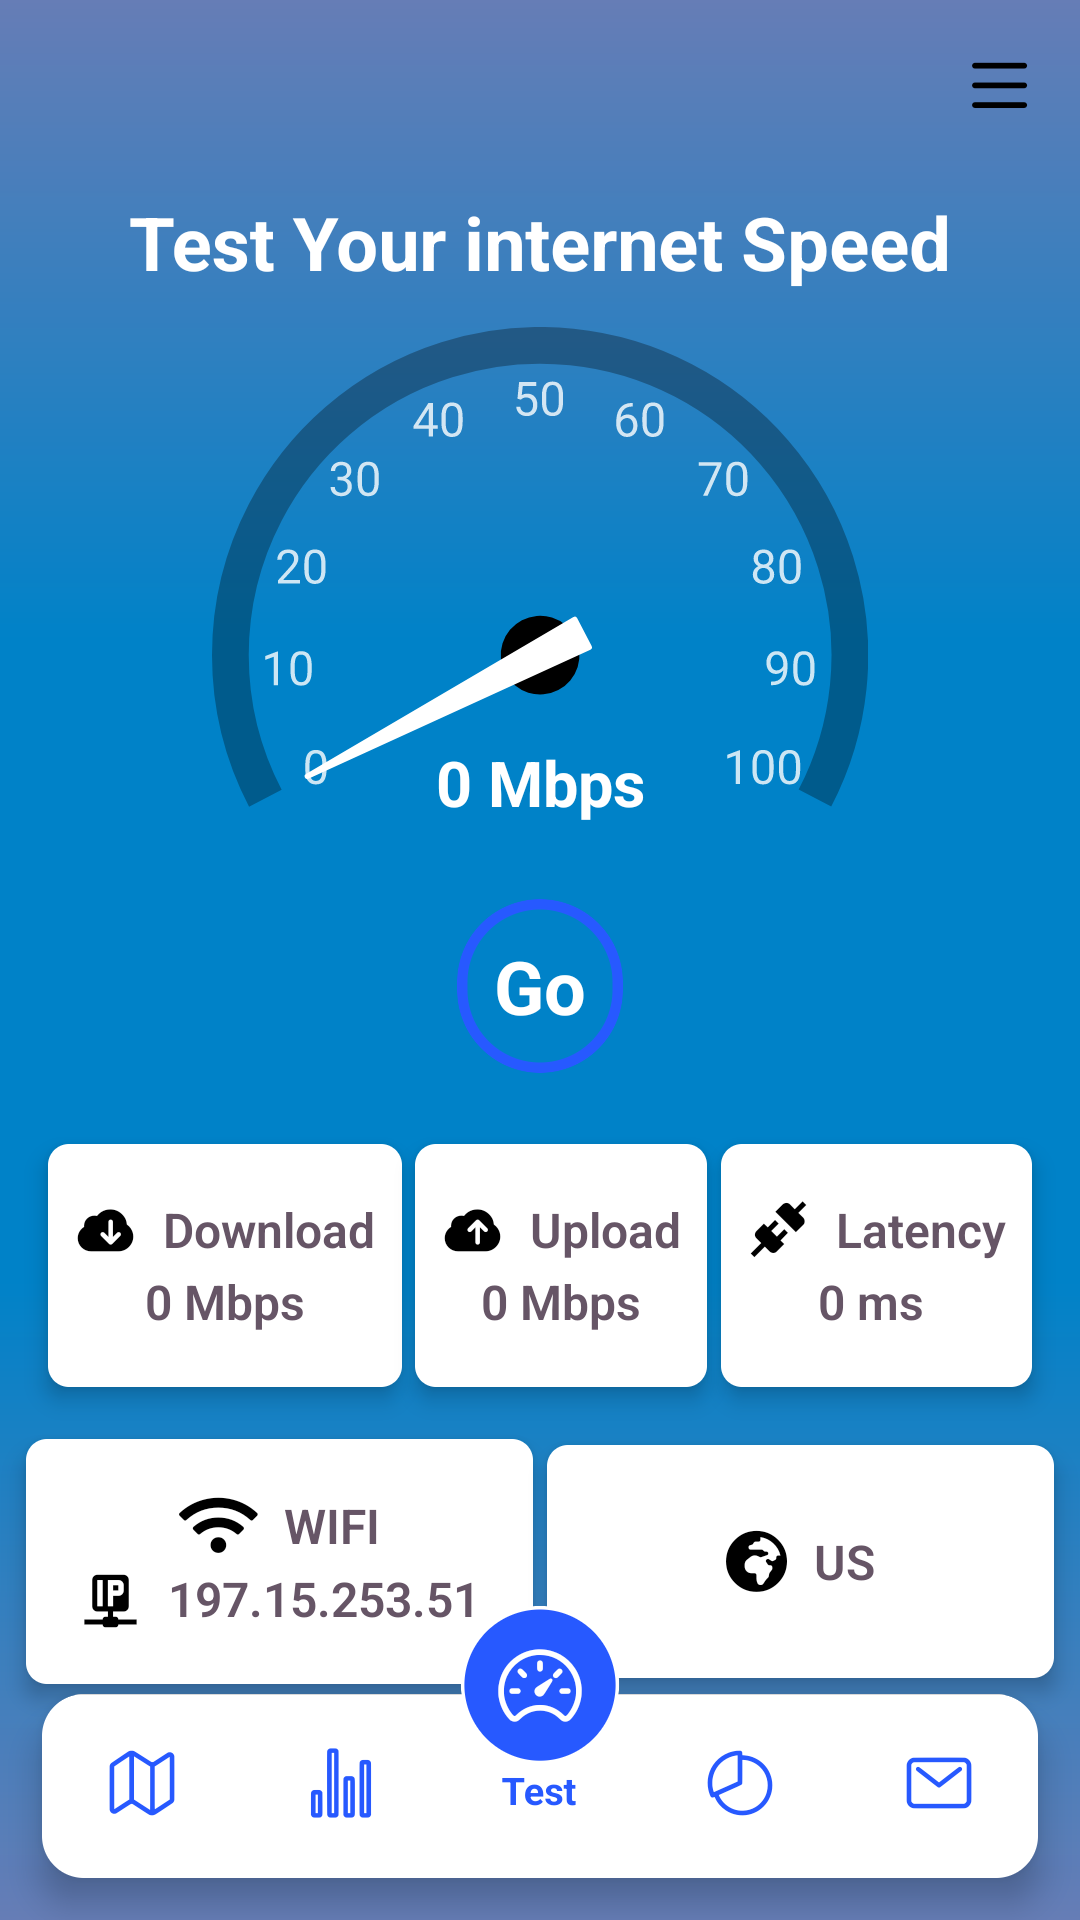
\includegraphics[width=\linewidth]{images/chap2/nav1.png}
    % \caption{Forget Password Sequence Diagram Part 1}
    \label{fig:login-form}
\end{minipage}\hfill
\begin{minipage}{0.3\textwidth}
    \centering
    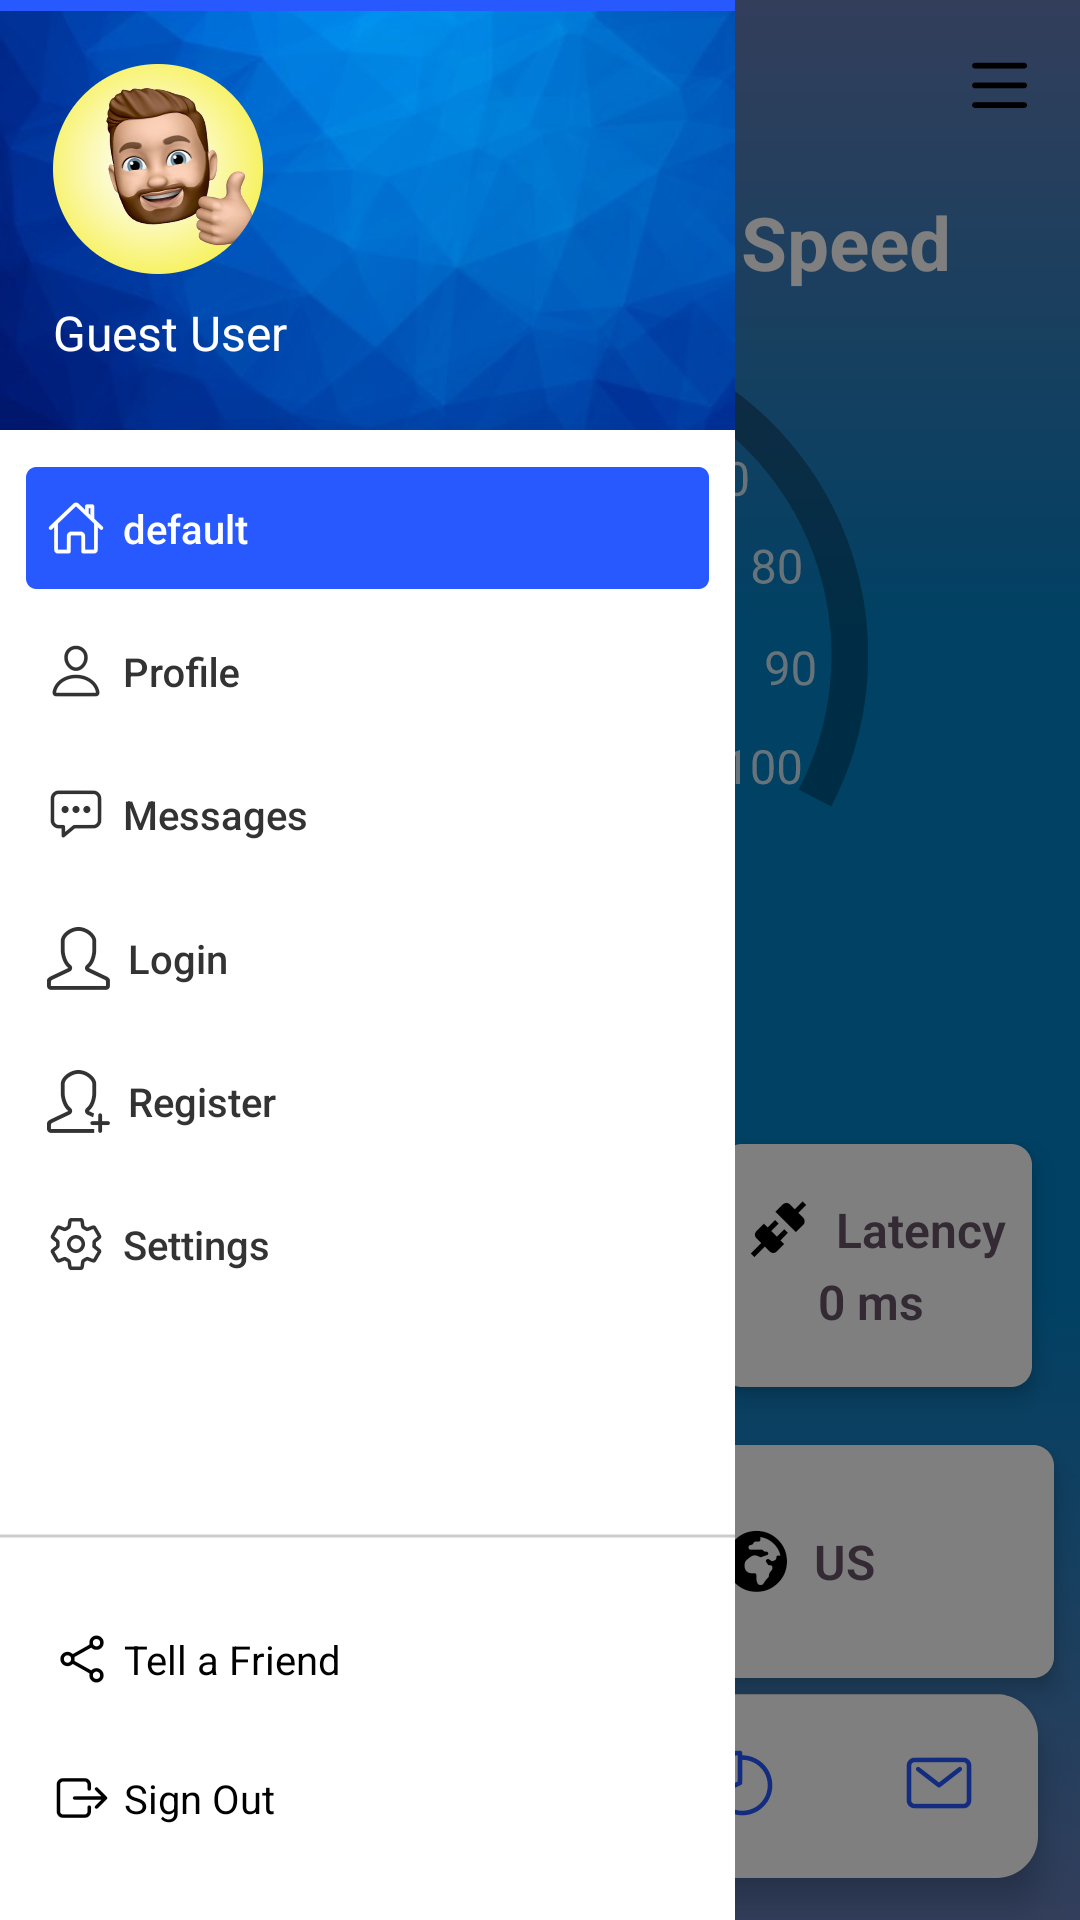
\includegraphics[width=\linewidth]{images/chap2/nav2.png}
    \label{fig:login-form-filled}
\end{minipage}
    \caption{Navigation system}
\end{figure}
\newpage
\section{User story n°3 : Authentication}
\subsection*{\textbf{\underline{Text description of the "Register" use case}}}
In the table below , we will have a clear idea about the  Register use case : 
\begin{table}[H]
    % \centering
    \renewcommand{\arraystretch}{1.5}  
   \begin{tabular}{|p{0.25\textwidth}|p{0.75\textwidth}|}
   \hline
        \textbf{Use Case} &  Register  \\   \hline
        
        \textbf{Actor(s) } & Guest User  \\   \hline
        \textbf{Pre-condition} &     
             The user requested the registration page
\\   \hline
        \textbf{Post-condition} & User will be redirected to the home page  \\  \hline

                \textbf{Principal scenario} & 
                \begin{enumerate}[left=0pt]
                \item The user requests the register screen .
                \item The system displays the registration page.
                \item The user enters his information.
                \item The user submits his information.
                \item The system validates the users information.
                \item The user is redirected to the home page.
                \end{enumerate}  \\   \hline
                 
          \textbf{Alternative\newline scenario} & 
      
             
             If the account  already exist , an error  message will appear to the user .\newline
            If an error related to the data occurs, a proper message will appear to the user to check his input.
 \\   \hline
\end{tabular}
  
         \caption{Text description of the “ Register” use case}
    \label{tab:my_label}
\end{table}

\newpage
\subsection*{\textbf{\underline{Text description of the "Login" use case}}}

\vspace{0.25cm}
In the table below , we will have a clear idea about the Login use case : 

\begin{table}[H]
    % \centering
    \renewcommand{\arraystretch}{1.5}
    
   \begin{tabular}{|p{0.25\textwidth}|p{0.7\textwidth}|}
   \hline
     
        \textbf{Use Case} & Login  \\   \hline
        
        \textbf{Actor(s) } & Registered User  \\   \hline
        \textbf{Pre-condition} &  
        \begin{itemize}[left=0pt]
             \renewcommand\labelitemi{\textbf{\Huge .}}
             
            \item The account has to be already created.
            \item The user requested the login page .
        \end{itemize} \\   \hline
        \textbf{Post-condition} & The use redirected to the previous page  \\  \hline
                \textbf{Principal scenario} & 
                \begin{enumerate}[left=0pt]
                \item The user requests the login screen .
                \item The system displays the login page.
                \item The user enter his information.
                \item The user submits his information.
                \item The system validates the users information.
                \item The user is redirected to the Test page.
                \end{enumerate}  \\   \hline                 
          \textbf{Alternative\newline scenario} & 
        \begin{itemize}[left=0pt]
             \renewcommand\labelitemi{\textbf{\Huge .}}
            \item If the account  does not exist , an error  message will appear to the user .
            \item If an error related to the data occurs , a proper message will appear to the user to check his input.
        \end{itemize} \\   \hline

\end{tabular}  
         \caption{Text description of the “Login” use case}
    \label{tab:my_label}
\end{table}

\subsection*{\textbf{\underline{Text description of the "Forget Password " use case}}}

\vspace{0.25cm}
In the table below , we will have break down the Forget Password use case : 

\begin{table}[H]
    % \centering
    \renewcommand{\arraystretch}{1.5}
    
   \begin{tabular}{|p{0.25\textwidth}|p{0.7\textwidth}|}
   \hline
     
        \textbf{Use Case} &Forget password  \\   \hline
        
        \textbf{Actor(s) } & Registered user  \\   \hline
        \textbf{Pre-condition} &  
        \begin{itemize}[left=0pt]
             \renewcommand\labelitemi{\textbf{\Huge .}}
            \item The account has to be already created
        \end{itemize} \\   \hline


        \textbf{Post-condition} & User's password is updated \\  \hline

                \textbf{Principal scenario} & 
                \begin{enumerate}[left=0pt]
                \item The user enter his email  .
                \item The system sends a verification mail that contains a secret code, to the provided email by the user  .
                \item The user submits the code .
                \item The system checks the code .
                \item The system displays a reset password form.
                \item The user fill the form with password and confirm password
                \item The system updates the database.
                \item A success message is displayed and the user is asked to login.
                \end{enumerate}  \\   \hline
                 
          \textbf{Alternative\newline scenario} & 
        \begin{itemize}[left=0pt]
             \renewcommand\labelitemi{\textbf{\Huge .}}
            \item If the account does not exist a warning message appears .
            \item If code is wrong a warning message appears and the user can ask for an other verification code.
            \item If the input is wrong the user is asked to check again.
            \item If the password is the same as the already saved in the database the user get warned.
        \end{itemize} \\   \hline
\end{tabular}
  
         \caption{Text description of the “Forget Password” use case}
    \label{tab:my_label}
\end{table}
% To realisation section
% 
% 

% Class diagram

% ###########################
% Sequence Diag
% 
% 
% ###########################
\subsection{Sequence Diagrams}
\subsubsection{Register Sequence Diagram}
\begin{figure}[H]
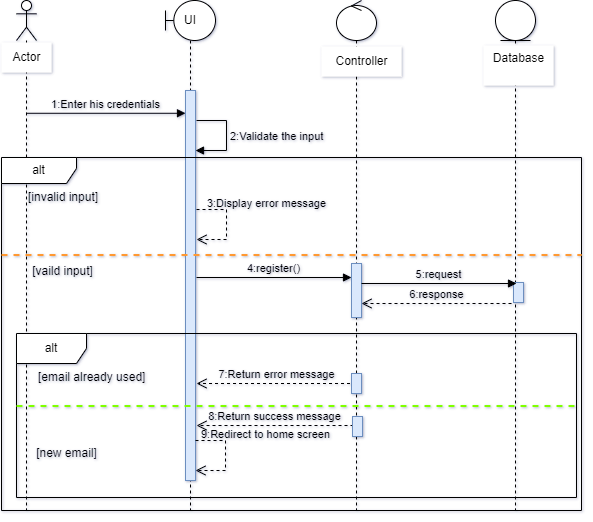
\includegraphics[width=0.98\textwidth]{images/chap2/registerSeq_c.png}
    \caption{“Register” Sequence Diagram}
    \label{fig:enter-label}    
\end{figure}
% ###########################
\subsubsection{Login Sequence Diagram}
\begin{figure}[H]
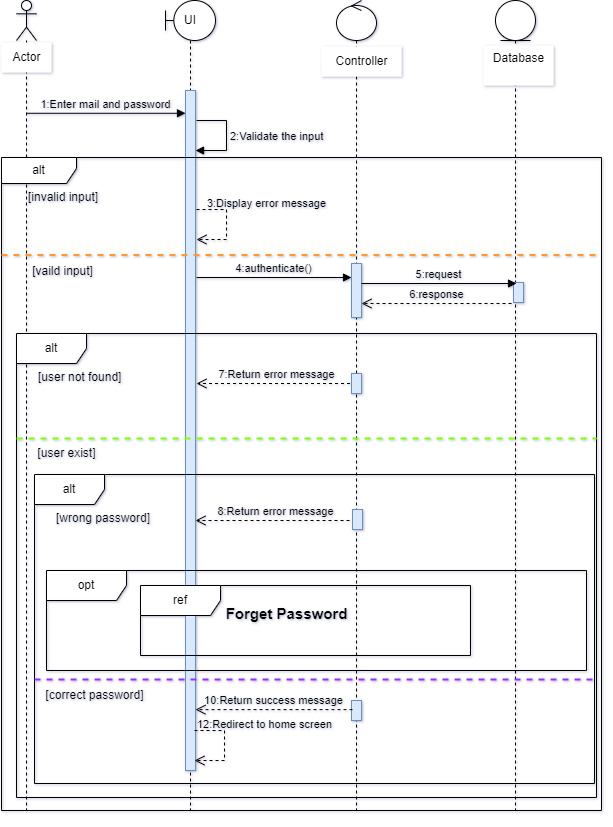
\includegraphics[width=0.98\textwidth]{images/chap2/AuthSeq_c.png}
    \caption{“Login” Sequence Diagram}
    \label{fig:enter-label}
\end{figure}

% ###########################
\subsubsection{Forget password  Sequence Diagram}
\begin{figure}[H]
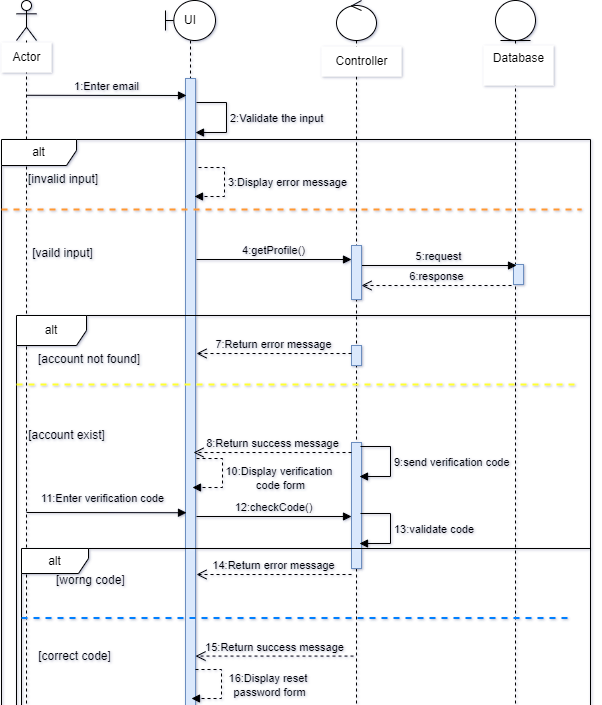
\includegraphics[width=0.98\textwidth]{images/chap2/resetPassword_cp1.png}
    % \caption{“Forget Password” Sequence Diagram}
    \label{fig:enter-label}    
\end{figure}
\begin{figure}[H]
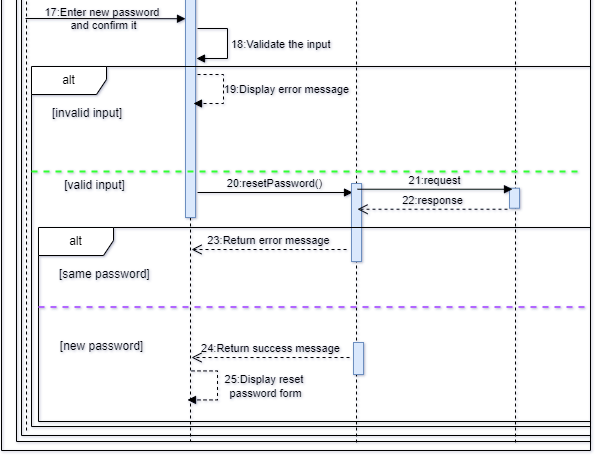
\includegraphics[width=0.98\textwidth]{images/chap2/resetPassword_cp2.png}
    \caption{“Forget Password” Sequence Diagram}
    \label{fig:enter-label}    
\end{figure}
% ###########################
\subsection{Class diagram }
Here is the class diagram that describes User entity in our database
\begin{figure}[H]
\begin{center}
    
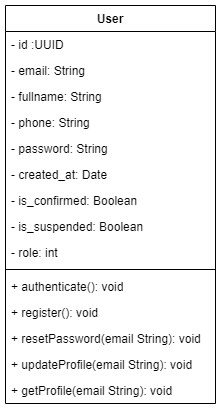
\includegraphics[width=0.3\textwidth]{images/chap2/userClass.png}
    \caption{Class diagram}
    \label{fig:enter-label} 
\end{center}
\end{figure}
% 
% 
% 
\subsection{Realization}
\subsubsection{Access Token and Refresh Token mechanism}
The authentication state of a user is generally represented by a token that is stored in some secured place in the application,this is the convention often used in the software industry ,in this application we used the JWT tokens to hold the user's authentication state .
For better securing our application we implemented a common mechanism of access/refresh token that's described by the figure below :
\begin{figure}[H]
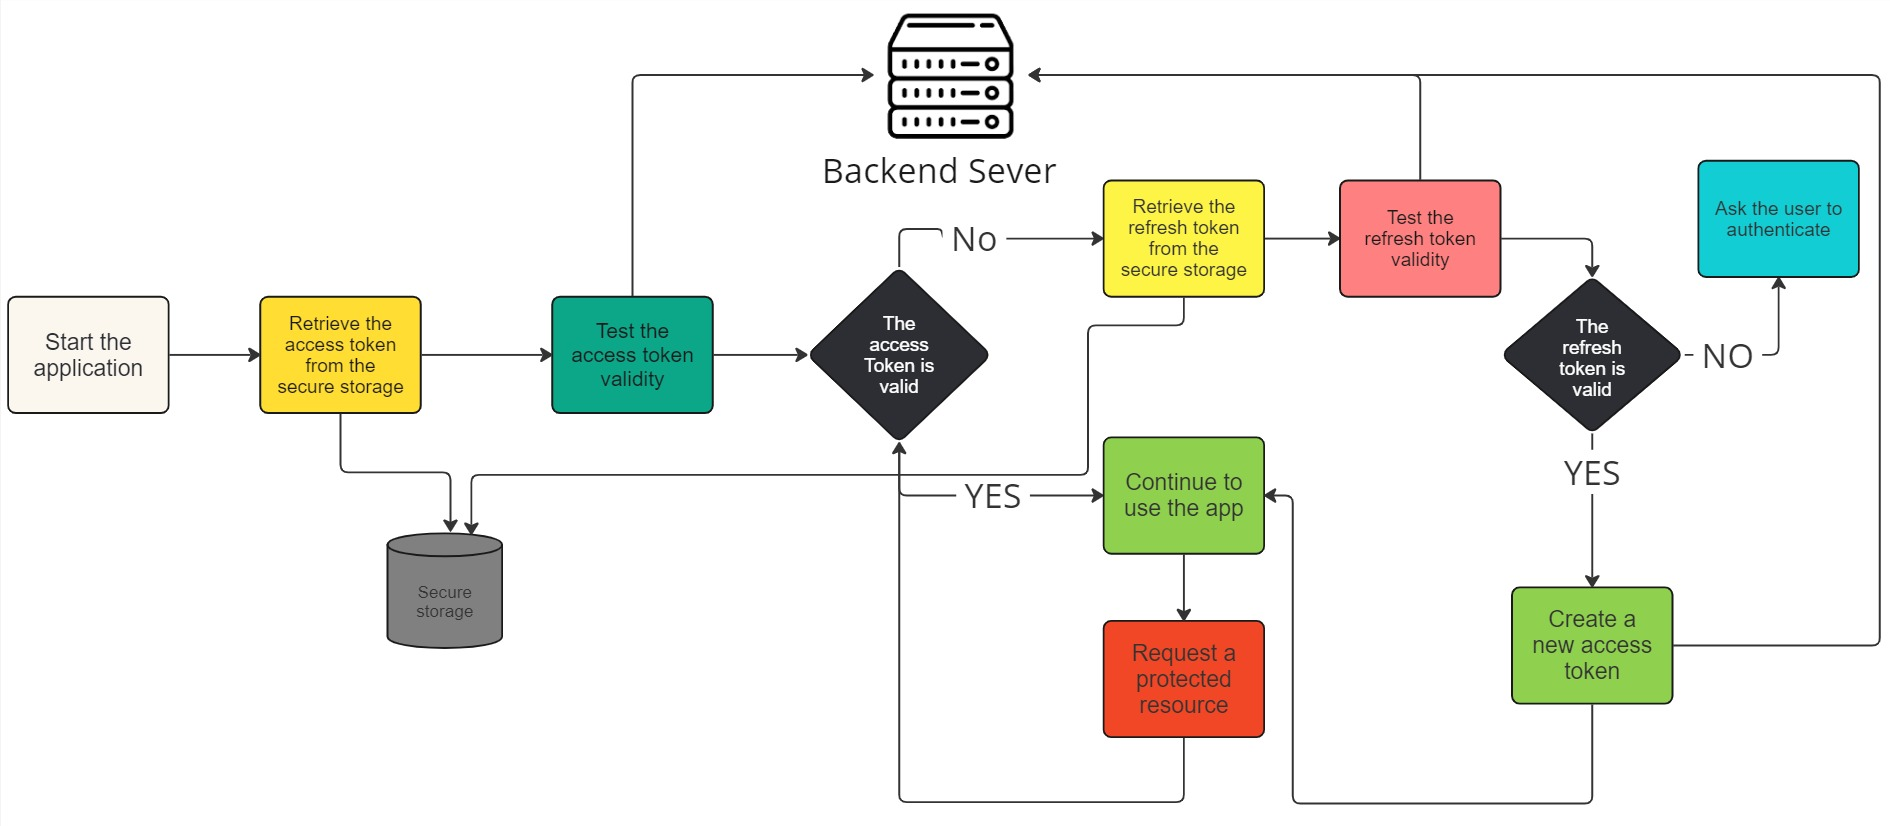
\includegraphics[width=1\textwidth]{images/chap2/refTkn.jpg}
    \caption{Access token and refresh token mechanism}
    \label{fig:enter-label}
\end{figure}
\subsubsection{Registration}
This is the interface that the user can create within 
\begin{figure}[H]
\begin{minipage}{0.45\textwidth}
    \centering
    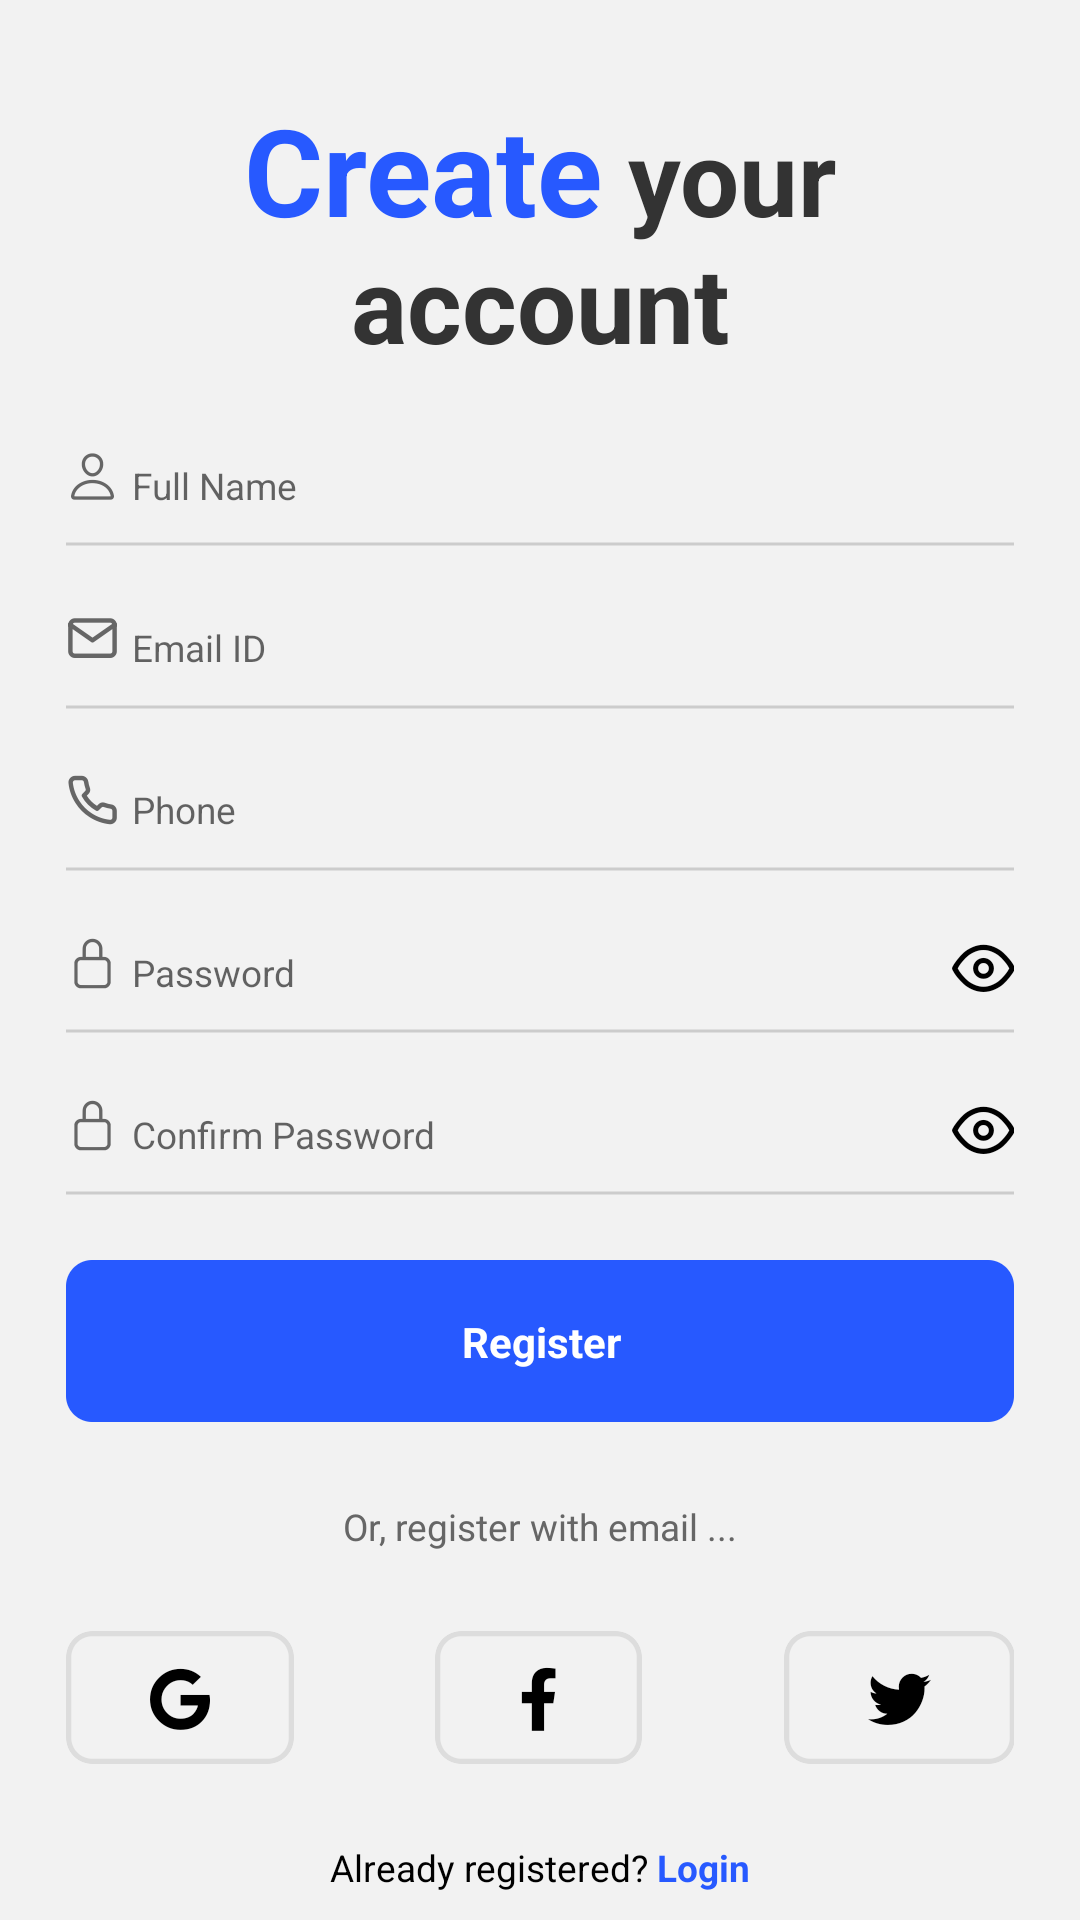
\includegraphics[width=\linewidth]{images/chap2/RegisterForm.png}
    \label{fig:login-form}
\end{minipage}\hfill
\begin{minipage}{0.45\textwidth}
    \centering
    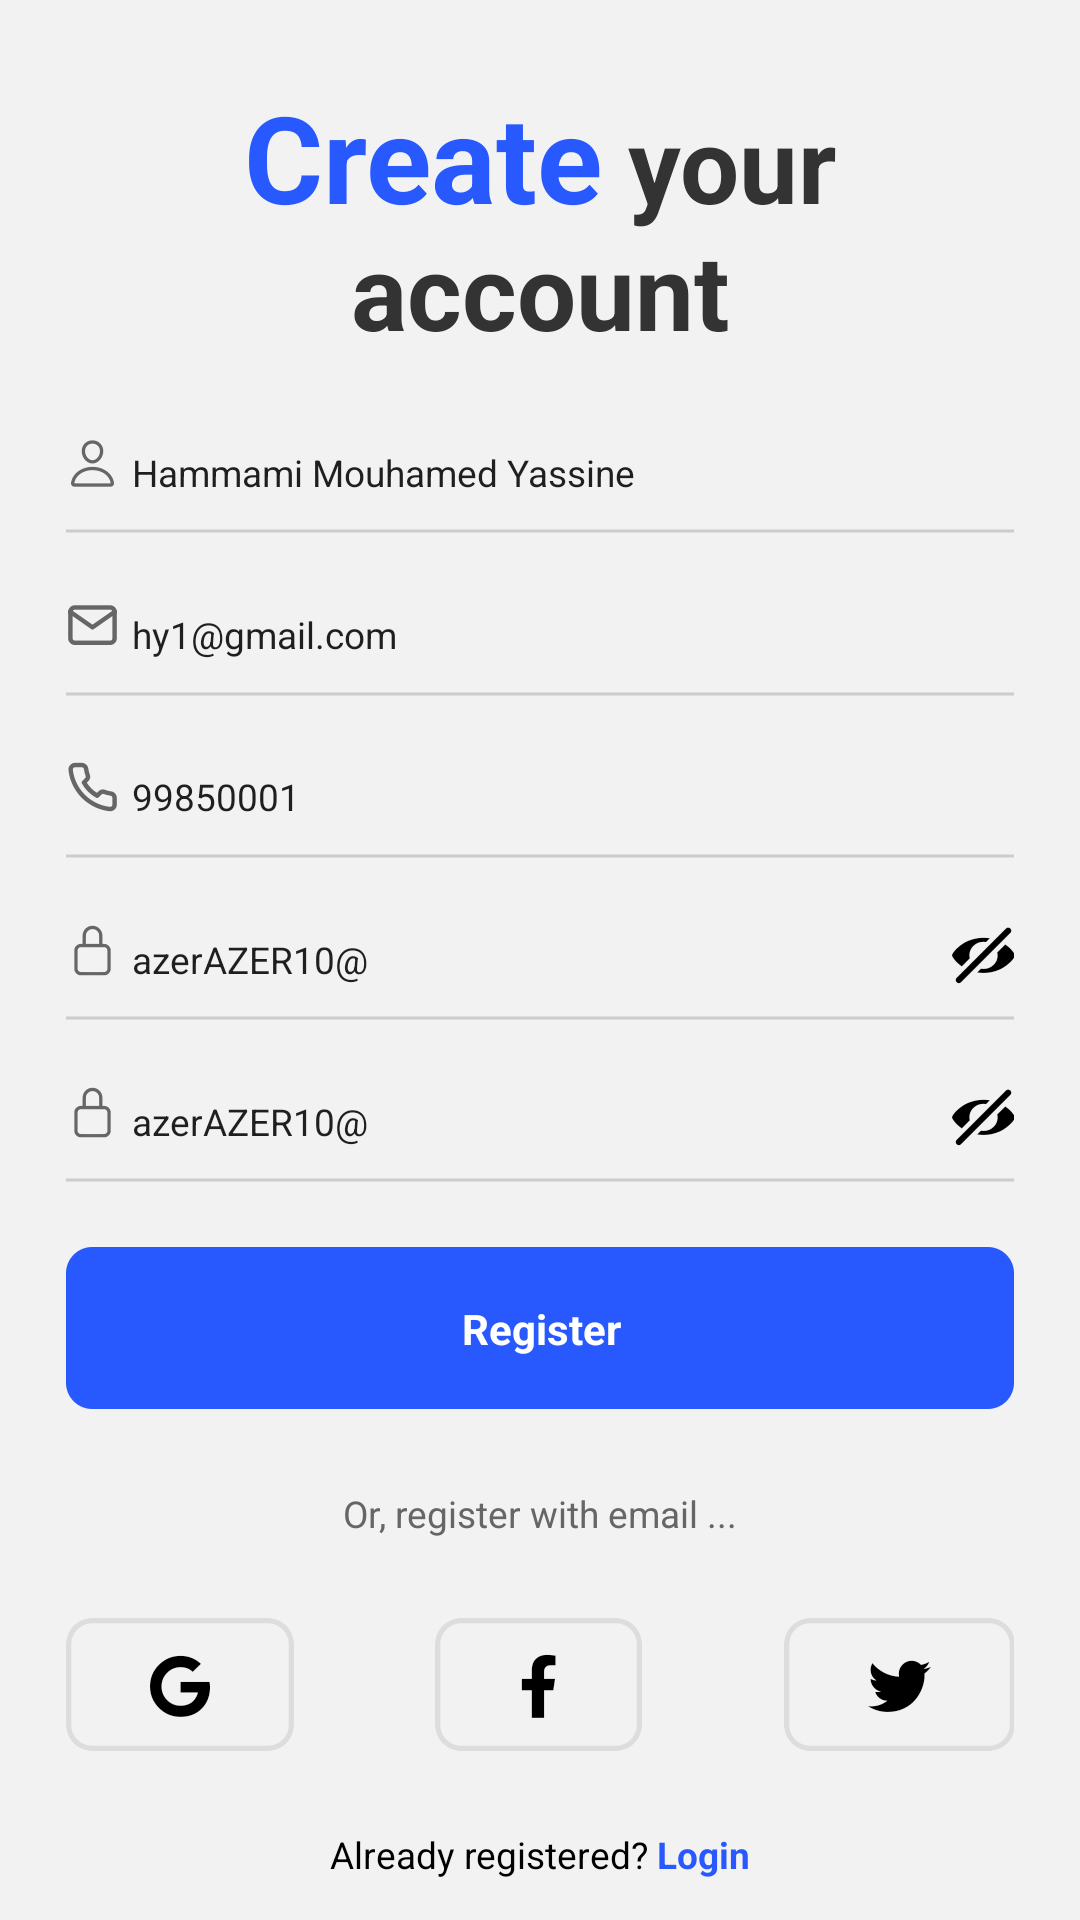
\includegraphics[width=\linewidth]{images/chap2/RegisterFormFilled.png}
    % \caption{Forget Password Sequence Diagram Part 2}
    \label{fig:login-form-filled}
\end{minipage}
    \caption{Registration user interface}
\end{figure}
% ###############
\newpage
\subsubsection{Authentication}
Via this interface the user can enter his credentials and authenticate to the application 
\begin{figure}[H]
\begin{minipage}{0.45\textwidth}
    \centering
    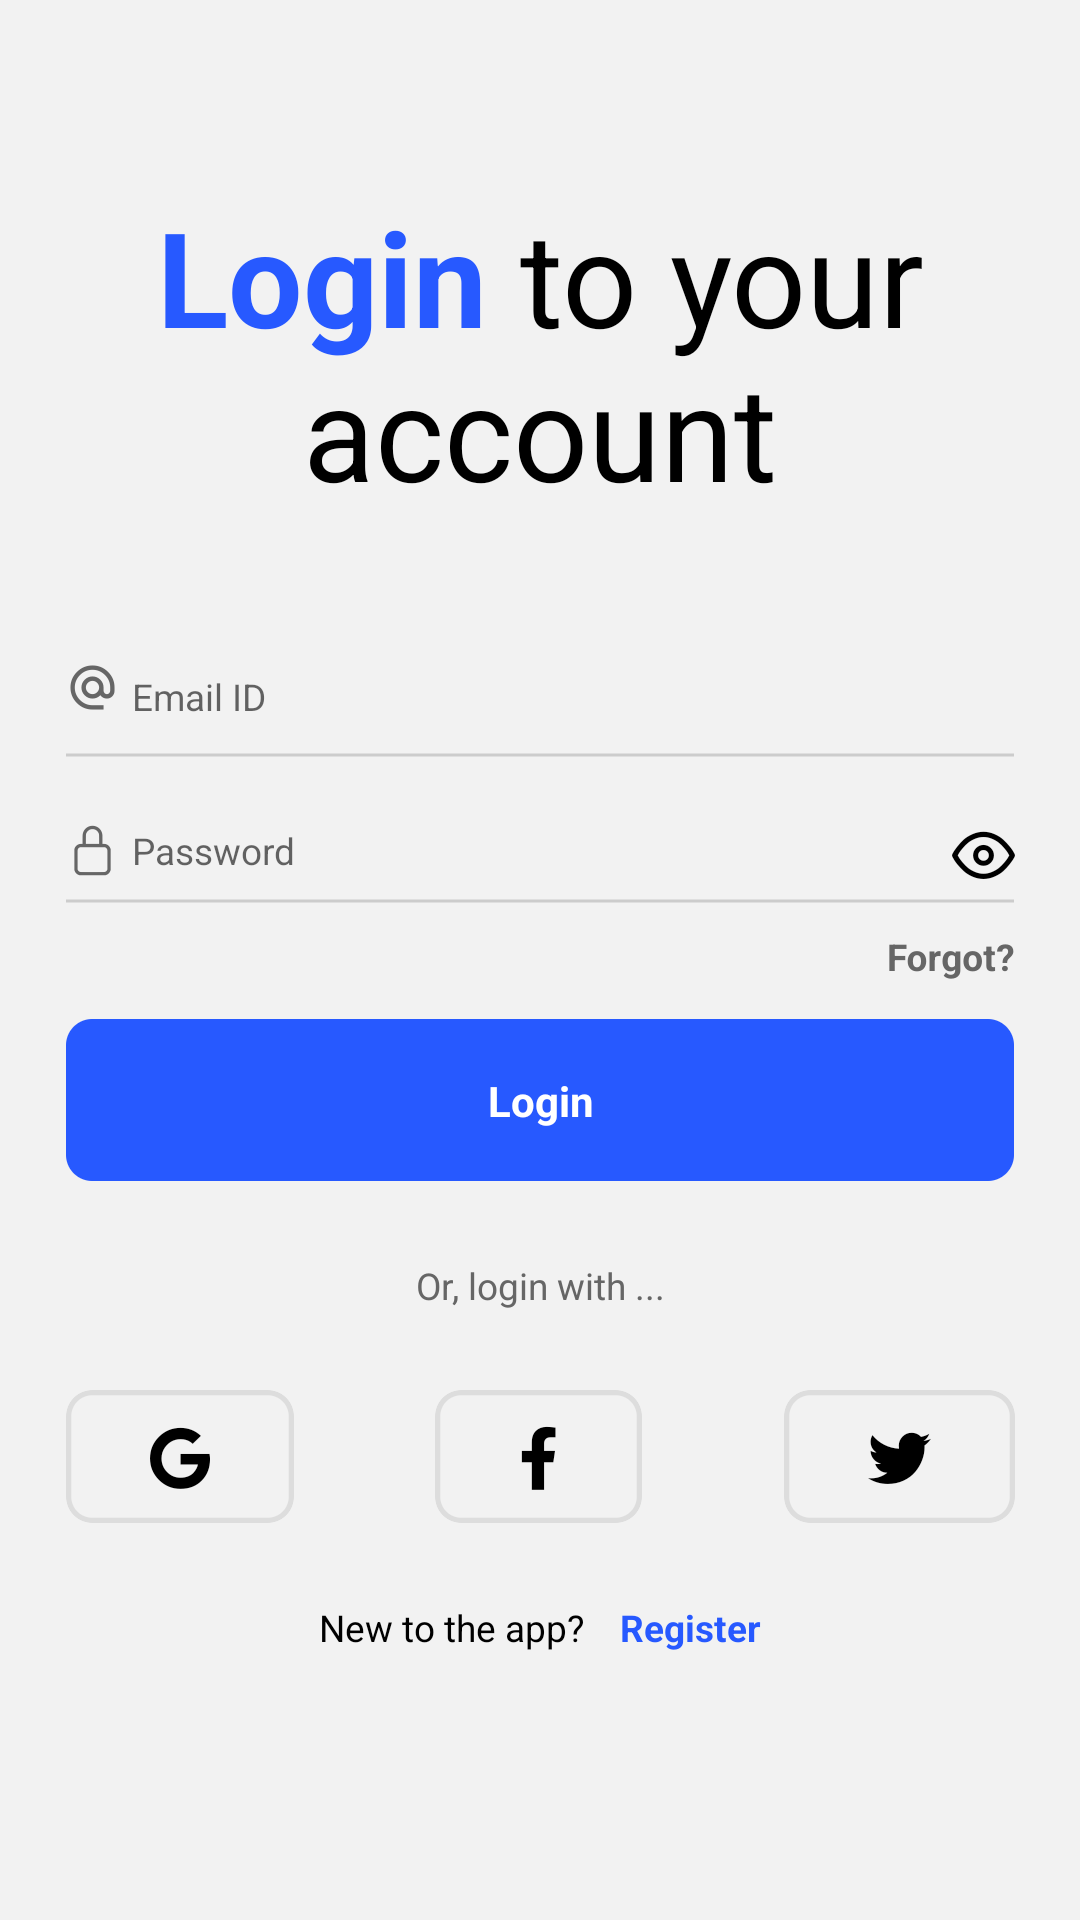
\includegraphics[width=\linewidth]{images/chap2/LoginForm.png}
    % \caption{Forget Password Sequence Diagram Part 1}
    \label{fig:login-form}
\end{minipage}\hfill
\begin{minipage}{0.45\textwidth}
    \centering
    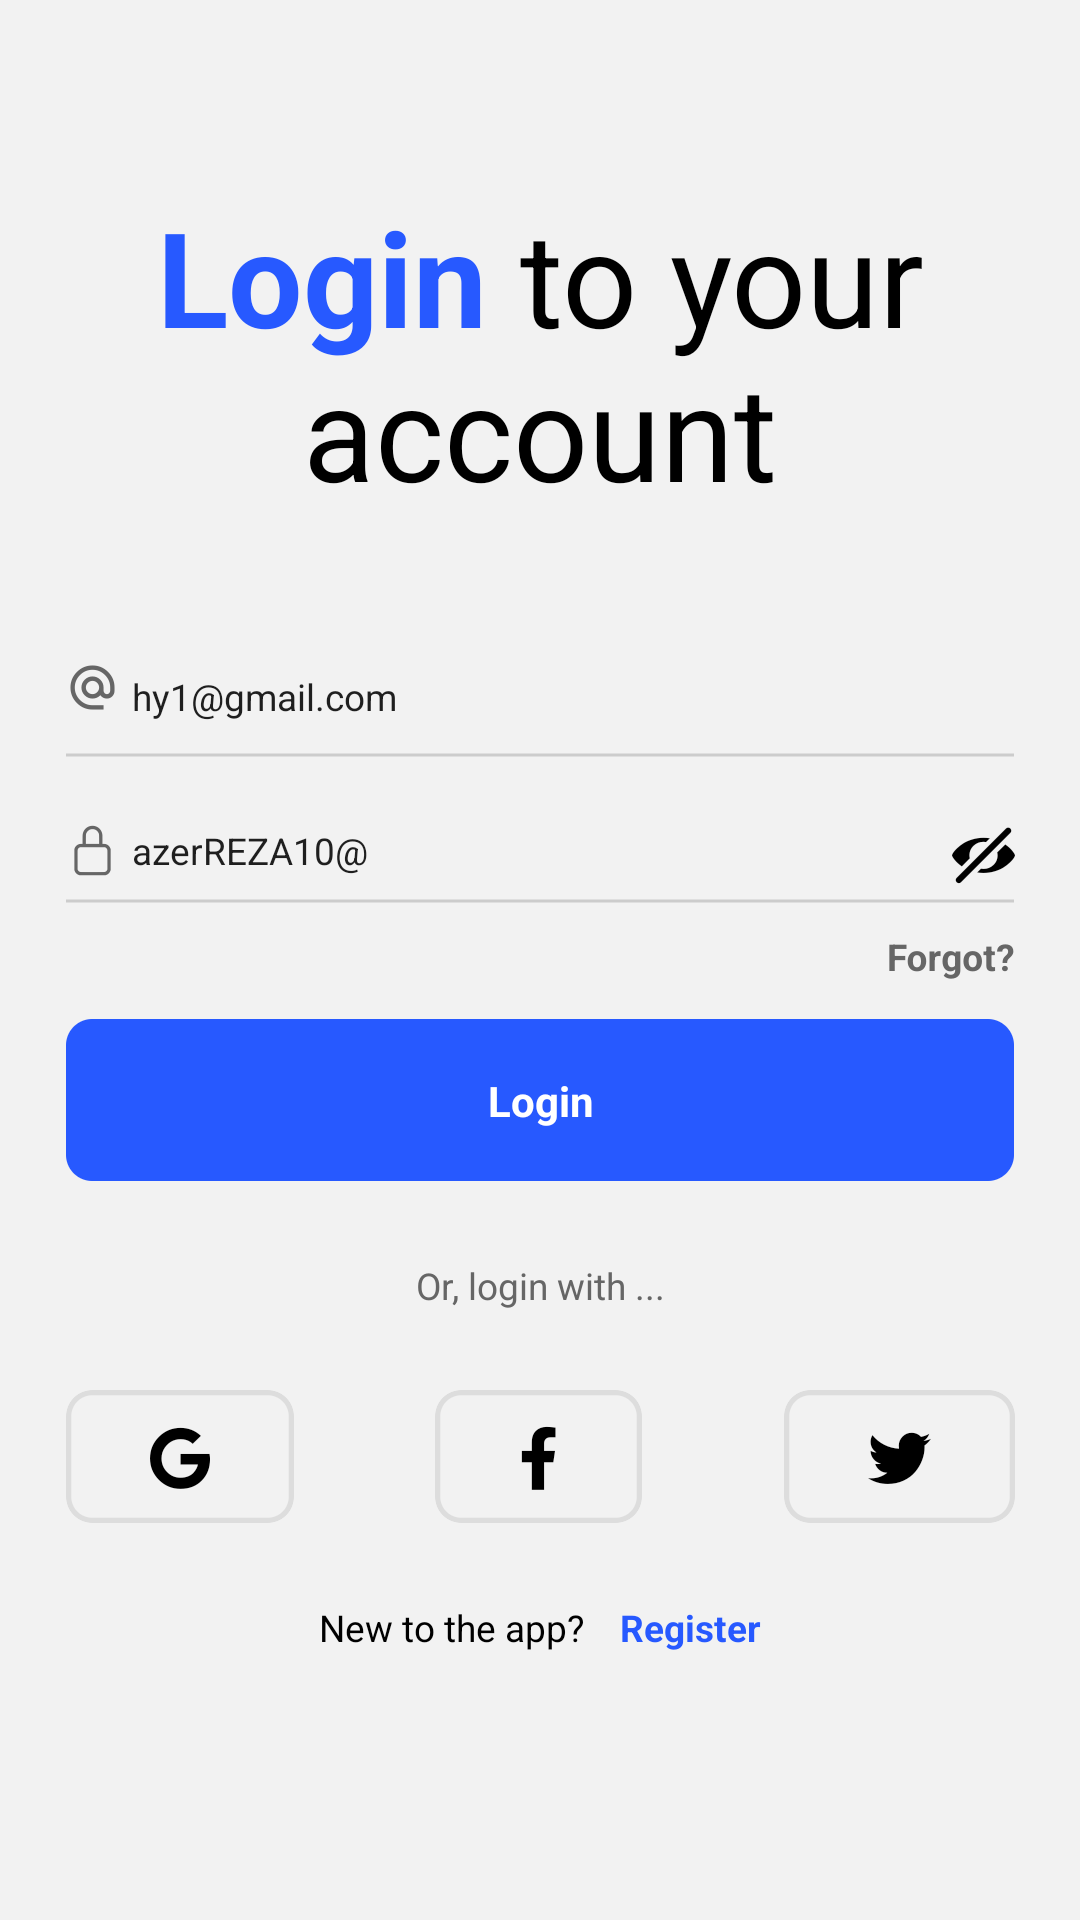
\includegraphics[width=\linewidth]{images/chap2/LoginFormFilled.png}
    \label{fig:login-form-filled}
\end{minipage}
    \caption{Login user interface}
\end{figure}
% ###########################
\newpage
\section{User story n°4 : Profile management}
\subsection*{\textbf{\underline{Text description of the "Update Credentials" use case}}}

\vspace{0.25cm}
In the table below , we will explain the Update Credentials use case : 

\begin{table}[H]
    % \centering
    \renewcommand{\arraystretch}{1.5}
    
   \begin{tabular}{|p{0.25\textwidth}|p{0.68\textwidth}|}
   \hline
     
        \textbf{Use Case} &Update Credentials  \\   \hline
        
        \textbf{Actor(s) } & Registered User  \\   \hline
        \textbf{Pre-condition} &  
        \begin{itemize}[left=0pt]
             \renewcommand\labelitemi{\textbf{\Huge .}}
            \item The user has to be authenticated 
            \item The user request the profile page 
        \end{itemize} \\   \hline


        \textbf{Post-condition} & User's profile is updated \\  \hline

                \textbf{Principal scenario} & 
                \begin{enumerate}[left=0pt]
                \item The user requests the profile page
                \item The system displays the profile page
                \item The user enters his new credentials
                \item The user confirms the modification
                \item The system updates the user credentials .
                \item The system displays the new credentials .
                \end{enumerate}  \\   \hline
                 
          \textbf{Alternative\newline scenario} & 
        \begin{itemize}[left=0pt]
             \renewcommand\labelitemi{\textbf{\Huge .}}
            \item If the input is wrong a warning message appears .

        \end{itemize} \\   \hline
\end{tabular}
         \caption{Text description of the “Update Credentials” use case}
    \label{tab:my_label}
\end{table}

\newpage
\subsection*{\textbf{\underline{Text description of the "Update Password" use case}}}

\vspace{0.25cm}
In the table below , we will explain the Update Password use case : 

\begin{table}[H]
    % \centering
    \renewcommand{\arraystretch}{1.5}
    
   \begin{tabular}{|p{0.25\textwidth}|p{0.68\textwidth}|}
   \hline
     
        \textbf{Use Case} &Update Password  \\   \hline
        
        \textbf{Actor(s) } & Registered User  \\   \hline
        \textbf{Pre-condition} &  
        \begin{itemize}[left=0pt]
             \renewcommand\labelitemi{\textbf{\Huge .}}
            \item The user has to be authenticated 
            \item The user request the profile page 
        \end{itemize} \\   \hline


        \textbf{Post-condition} & User's password is updated \\  \hline

                \textbf{Principal scenario} & 
                \begin{enumerate}[left=0pt]
                \item The user requests the profile screen
                \item The user requests the change password screen
                \item The system displays the change password screen
                \item The user enters his new password and confirm it 
                \item The user confirms the modification
                \item The system updates the user's password
                \end{enumerate}  \\   \hline
                 
          \textbf{Alternative\newline scenario} & 
        \begin{itemize}[left=0pt]
             \renewcommand\labelitemi{\textbf{\Huge .}}
            \item If the input is wrong a warning message appears .
            \item If the password is similar to the old one, a failure message appears.
        \end{itemize} \\   \hline
\end{tabular}
         \caption{Text description of the “Update Password” use case}
    \label{tab:my_label}
\end{table}
\subsection{Sequence diagram}
\begin{figure}[H]
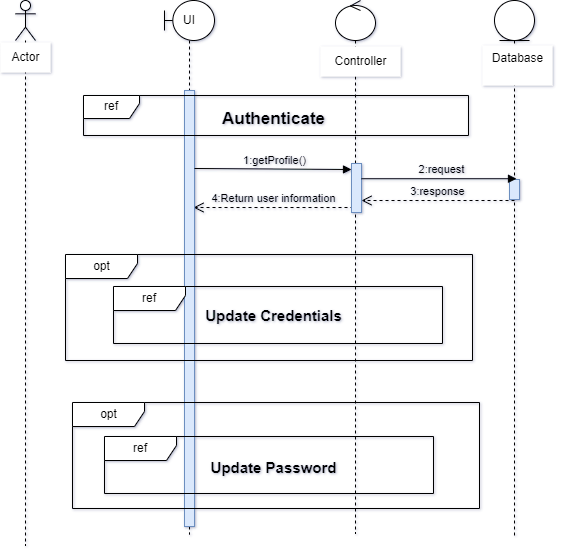
\includegraphics[width=0.98\textwidth]{images/chap2/manageProfile_c.png}
    \caption{“Manage Profile” sequence Diagram}
    \label{fig:enter-label}    
\end{figure}
\begin{figure}[H]
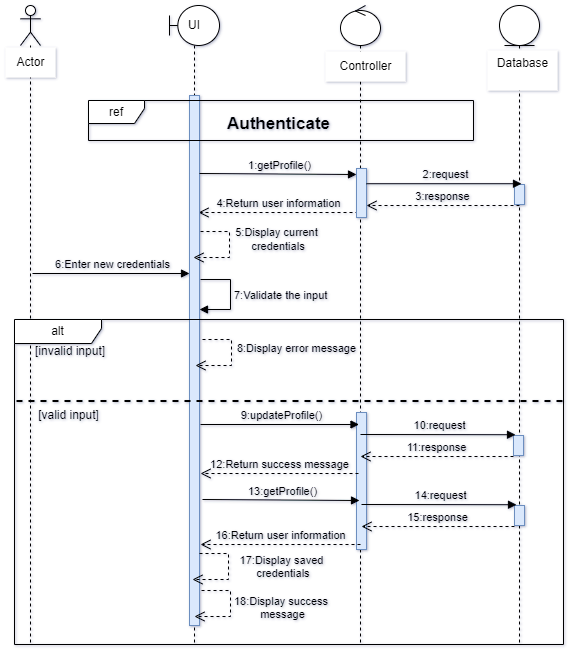
\includegraphics[width=0.98\textwidth]{images/chap2/updateCred.png}
    \caption{“Update Credentials” sequence Diagram}
    \label{fig:enter-label}    
\end{figure}
\begin{figure}[H]
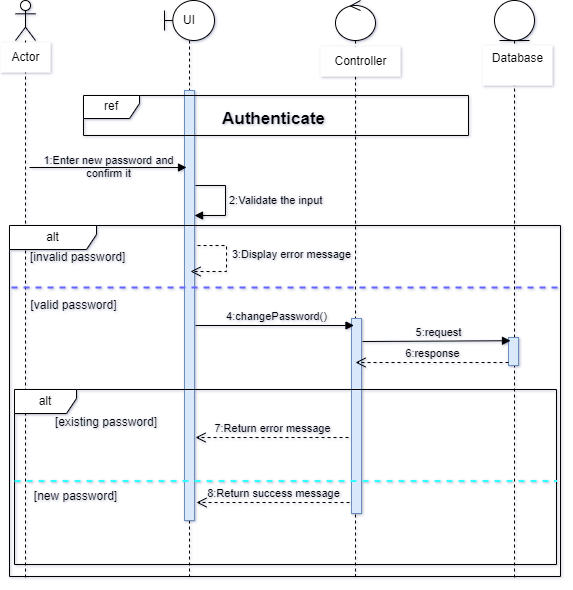
\includegraphics[width=0.98\textwidth]{images/chap2/changePassword_c.png}
    \caption{“Update Password” sequence Diagram}
    \label{fig:enter-label}    
\end{figure}
% 
% 
% 
\newpage
\subsection{Realization}
% ###############
\subsubsection{Manage Profile interfaces}
Via this interface the user can update information related to his profile like credentials and password
\begin{figure}[H]
\begin{minipage}{0.45\textwidth}
    \centering
    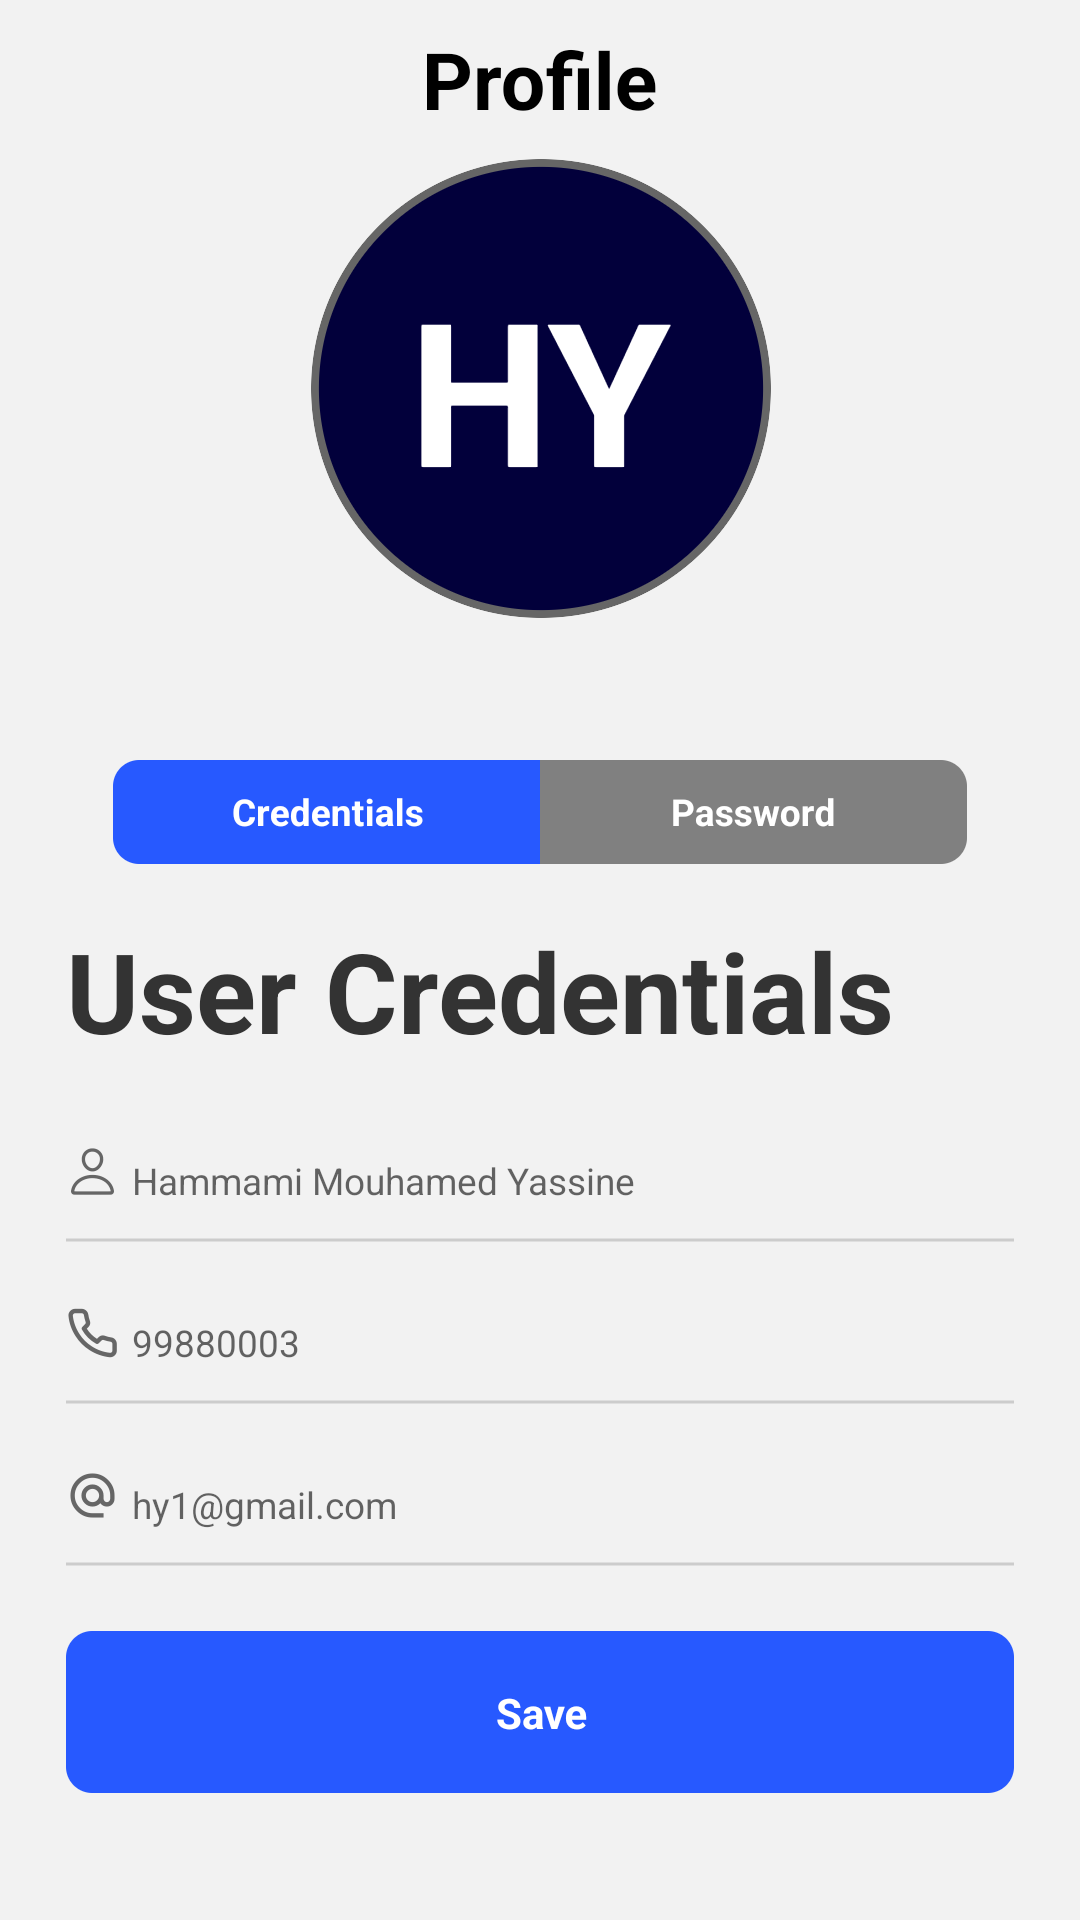
\includegraphics[width=\linewidth]{images/chap2/editUserCred.png}
    % \caption{Forget Password Sequence Diagram Part 1}
    \label{fig:login-form}
\end{minipage}\hfill
\begin{minipage}{0.45\textwidth}
    \centering
    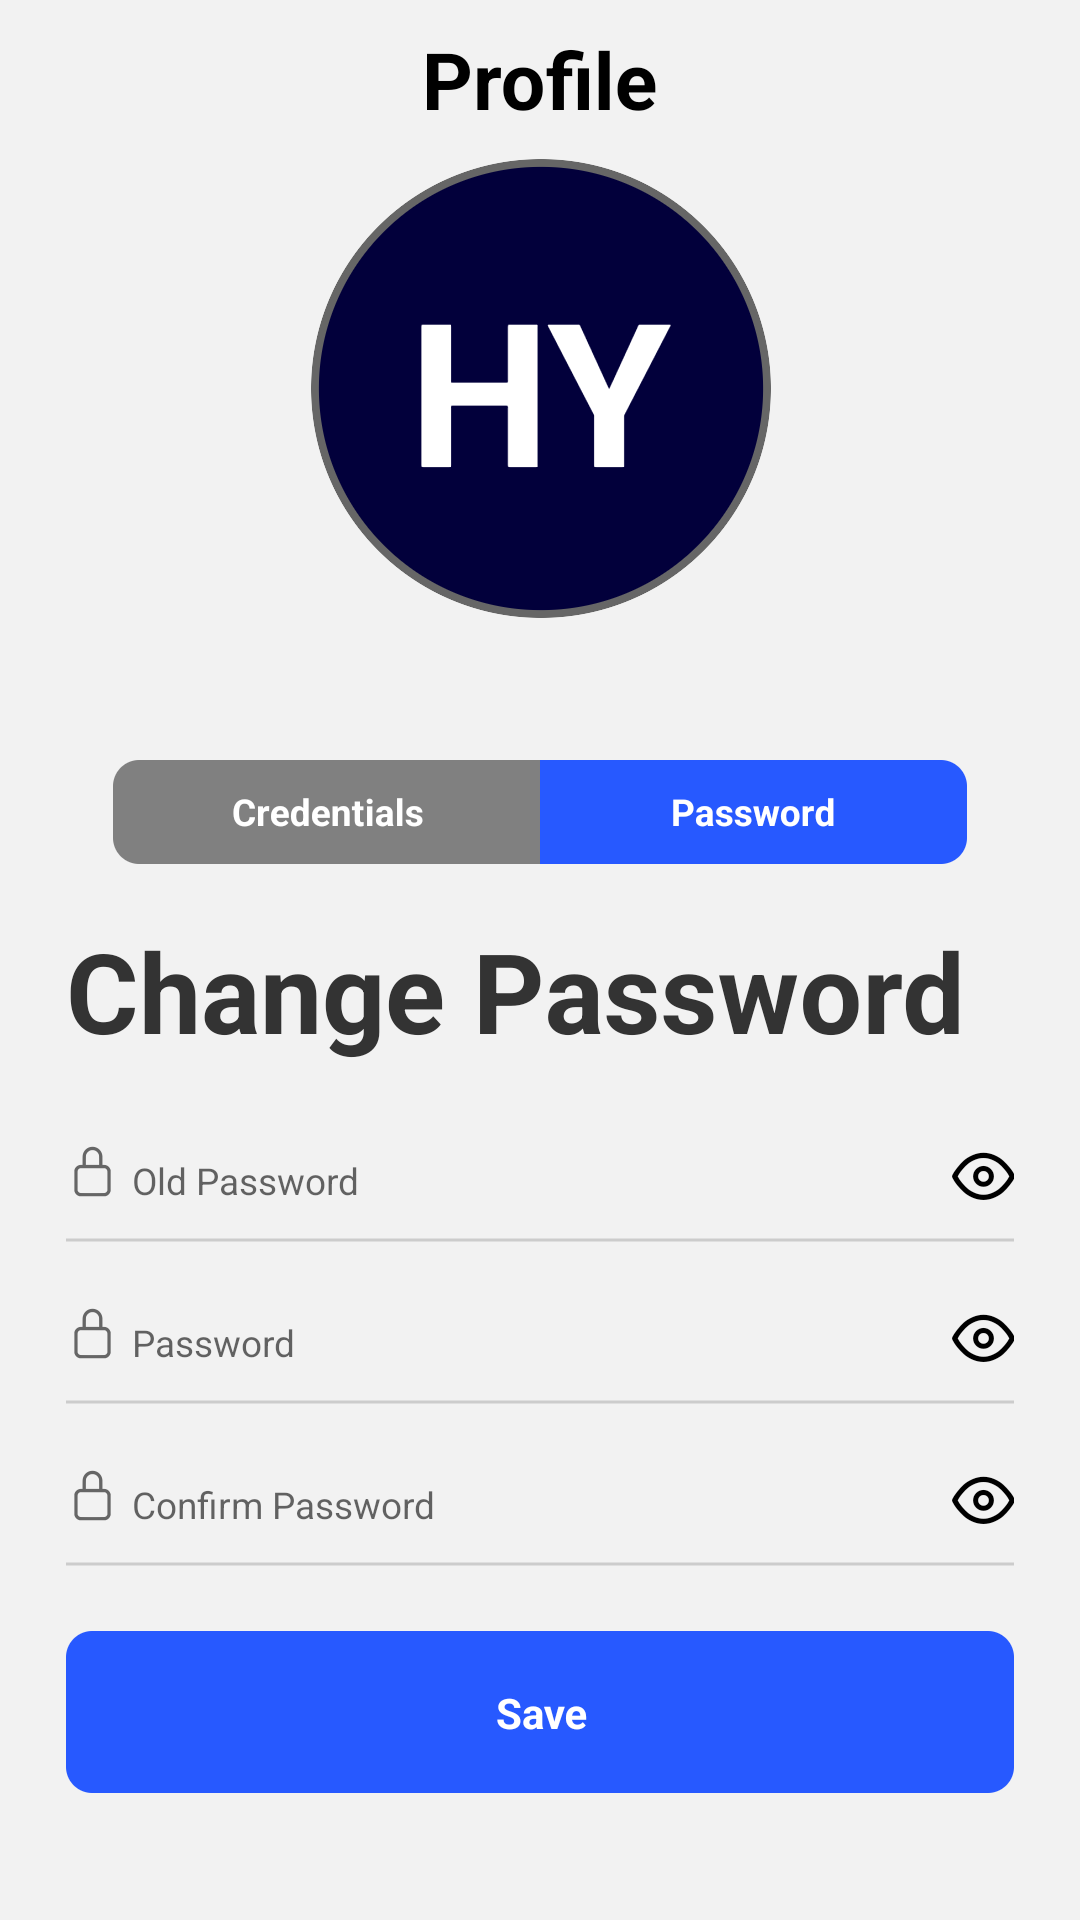
\includegraphics[width=\linewidth]{images/chap2/editPwd.png}
    \label{fig:login-form-filled}
\end{minipage}
    \caption{Manage Profile interfaces}
\end{figure}
\section*{Conclusion}
In this sprint we successfully implemented the skeleton of our application that's composed by configuration service ,the navigation system and the authentication system . In the next chapter we will target  the network testing and report generation  module 


\chapter*{Chapter 4}
\markboth{Sprint 2 : Network Testing \& Reports generation}{Sprint 2 : "Network Testing \& Reports generation} %pour afficher l'entete
 \addcontentsline{toc}{chapter}{4 Sprint 2 : Network Testing \& Reports generation}


\setcounter{chapter}{4}
\setcounter{section}{0}
\setcounter{table}{0} 
\setcounter{figure}{0} 


\etocsettocstyle{\subsection*{Plan}}{}
\vspace{0.25cm}

\setcounter{tocdepth}{1}
\headrule{
\vspace{0.5cm}

\begin{center}
    \textsc{\textbf {\Huge Sprint 2 : Network Testing \& Reports generation}} 
\end{center}
}
\headrule


\localtableofcontents
\newpage

\section*{Introduction}
After completing the first sprint and build the application's skeleton that we presented in the previous chapter, it's time to to go further and realize the rest of the functionalities .   
In this chapter, we will tackle the second sprint of our project which focuses on the "Network Testing \& Reports generation" .
We will cover its analysis, modeling, and realization.

\section{Sprint 2 Backlog}

The sprint backlog is a detailed list of tasks and user stories selected for completion within the current sprint, guiding the development team's work towards achieving the sprint goal. It serves as a dynamic, prioritized plan that evolves as the team progresses and new information emerges.
The table below describes the backlog of the second sprint :



\begin{table}[H]
    % \centering
    \renewcommand{\arraystretch}{1.2}
    \setlength{\belowcaptionskip}{0.25cm}
 
   \begin{tabular}{|p{0.05\textwidth}|p{0.2\textwidth}|p{0.34\textwidth}|p{0.34\textwidth}|}
   \hline
   \textbf{ID}  &  \textbf{User Story } & \textbf{Description} & \textbf{Task} \\ \hline


   
   \begin{center}
       \textbf{1}
   \end{center} & \begin{center}
       As a user, I want to test my network
   \end{center} &
   The user can perform a  network test and have results on network download and upload speed and latency, also he can  save the test result and give his evaluation.
   & 

       \begin{itemize}[left=0pt, label={\textbf{\Huge .}}]
       % \renewcommand\labelitemi{\textbf{\Huge .}}
            \item Develop the backend logic for testing the network
            \item Develop the user interface for  launching a test
            \item Develop the user interface for  saving result
            \item Develop the backend for managing  saved results
        \end{itemize} \\ \hline


   \begin{center}
       \textbf{2}
   \end{center} & \begin{center}
       As a  user, I want to inspect the reports based on my performed tests
   \end{center} &
   
  The  user can visit his testing history and visualize the variation of his network state based on different criteria like (internet provider , region , connection type,evaluation).  & 

       \begin{itemize}[left=0pt, label={\textbf{\Huge .}}]
            \item Develop the user interface to display the history
            \item Develop the user interface to display different charts 

        \end{itemize} \\ \hline
      
\end{tabular}
       \caption{Sprint 2 Backlog}
        \label{tab:my_label}
    
\end{table}



\newpage

\section{Sprint 2 use case diagram}

The figure below showcases the use case diagram for this sprint the involved actors and the expected functionalities  from our application.

\begin{figure}[H]
    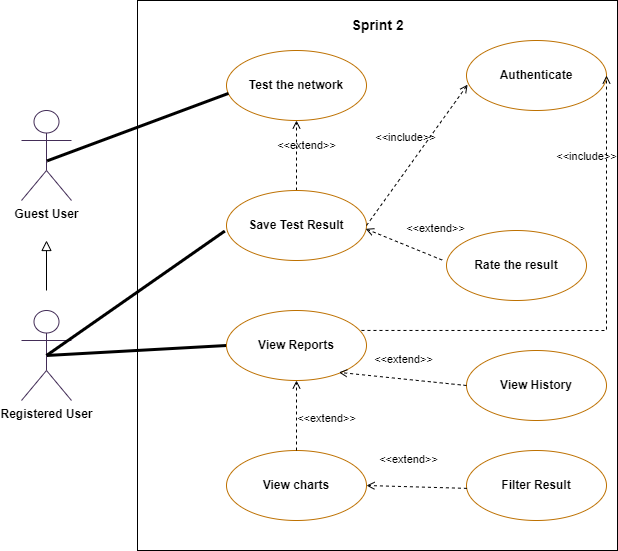
\includegraphics[width=0.98\textwidth]{images/sprint2/Sprint2UC.png}
     \caption{Sprint 2 Use Case Diagram}
    \label{fig:enter-label}
    
\end{figure}

\newpage
\section{User story n°1 : Network testing}
\textbf{\underline{Text description of the “Test the Network ” use case}}

\vspace{0.25cm}
We detail through this table the use case “Test the Network” :

\begin{table}[H]
    % \centering
    \renewcommand{\arraystretch}{1.5}
    
   \begin{tabular}{|p{0.25\textwidth}|p{0.68\textwidth}|}
   \hline
     
        \textbf{Use Case} & Test the network  \\   \hline
        
        \textbf{Actor(s) } & Guest user / Authenticated user   \\   \hline
        \textbf{Pre-condition} & 
           \begin{itemize}[left=0pt, label={\textbf{\Huge .}}]
            \item  The User request the testing page.
            \item  The device is connected to the internet.
        \end{itemize} 
        \\  \hline
        \textbf{Post-condition} & None \\   \hline


                \textbf{Principal scenario} &
                \begin{enumerate}[left=0pt]
                    \item The user launches the test.
                    \item The system retrieves some information about the user session (ip address,location,internet provider).
                    \item The system displays the retrieved data.
                    \item The system exchanges some chunks of data with the server .
                    \item After the receiving the last chunk of data, the system compute the metrics values.
                    \item The system displays the data and ask the user for saving the values in the database.
                    \item If the user confirms the values will sent to the database.
                
                    \end{enumerate}  \\   \hline

                     \textbf{Alternative\newline scenario} & 
        \begin{itemize}[left=0pt, label={\textbf{\Huge .}}]
            \item  If the device is not connected to the the internet a warning message appears.
        \end{itemize} \\   \hline
       
\end{tabular}

     \caption{Text Description Of The “Test the network” Use Case}
    \label{tab:my_label}
    
\end{table}

\newpage

\subsection{Sequence Diagram <<Test the network>> }



\begin{figure}[H]
   
    
    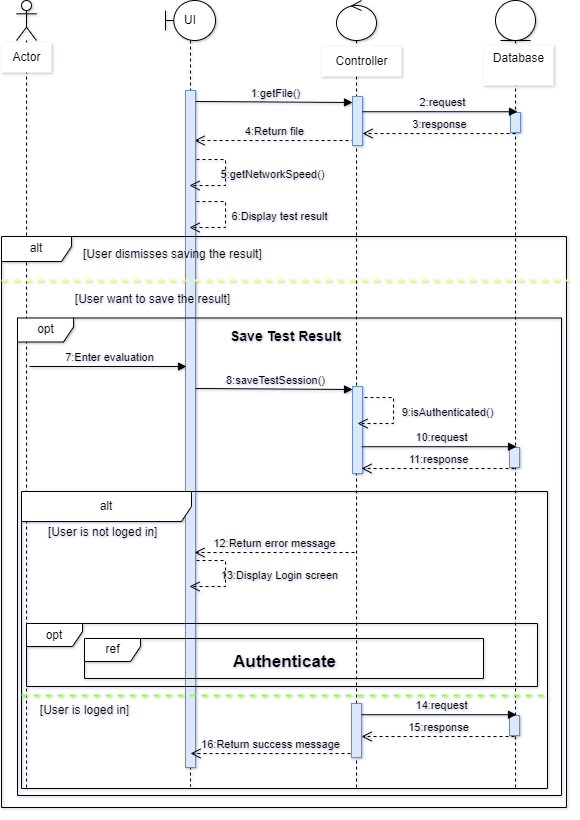
\includegraphics[width=0.98\textwidth]{images/sprint2/testNetworkSeq.png}
    \caption{“Test the network” Sequence Diagram}
    \label{fig:enter-label}
    
\end{figure}
\newpage
\subsection{Sprint 2 Class Diagram}
\begin{figure}[H]
   
    
    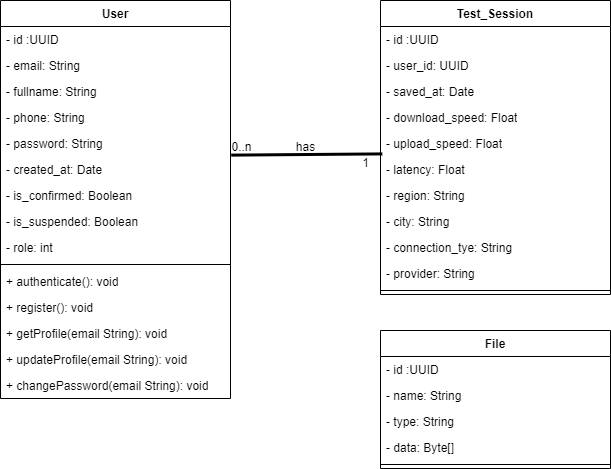
\includegraphics[width=0.98\textwidth]{images/sprint2/Sprint2ClassDiag.png}
    \caption{Sprint 2 Class Diagram}
    \label{fig:enter-label}
    
\end{figure}
\newpage
\subsection{Realization}
In the section we will explore the final user interfaces related to the user story n°1 : "Network Testing" in a sequential order :
\begin{figure}[H]
\begin{minipage}{0.32\textwidth}
    \centering
    \includegraphics[width=\linewidth]{images/sprint2/testModuleInit.png}
    \label{fig:login-form-filled}
\end{minipage}\hfill
\begin{minipage}{0.3\textwidth}
    \centering
    \includegraphics[width=\linewidth]{images/sprint2/testModuleActive.png}
    \label{fig:login-form}
\end{minipage}\hfill
\end{figure}
% \newpage
% After Finishing the test a modal like shown in the screen shot below appears
\begin{figure}[H]
\begin{center}
    \begin{minipage}{0.32\textwidth}
    \includegraphics[width=\textwidth]{images/sprint2/testModuleFinish.png}
    \label{fig:enter-label}
    \end{minipage}\hfill
    \caption{Testing Screen}
\end{center}
\end{figure}


\newpage
\section{User story n°2 : Report generation}

\textbf{\underline{Text description of the “View Reports”use case:}}

\vspace{0.25cm}

We detail through this table the use case “View Reports” :

\begin{table}[H]
    % \centering
    \renewcommand{\arraystretch}{1.5}
    
   \begin{tabular}{|p{0.25\textwidth}|p{0.68\textwidth}|}
   \hline
     
        \textbf{Use Case} & View Reports  \\   \hline
        
        \textbf{Actor(s) } & Authenticated User  \\   \hline
        \textbf{Pre-condition} & The user requests the reports screen \\   \hline
        \textbf{Post-condition} & None  \\   \hline
                \textbf{Principal scenario} & 
                \begin{enumerate}
                    \item The user enters the reports screen.
                    \item The system retrieve the data related to the user .
                    \item The user interacts with the default charts.
                    \item The request an other chart.
                    \item The system extract the needed values and display the requested chart.
                \end{enumerate}  \\   \hline
        
        \textbf{Alternative\newline scenario} & 
        \begin{center}
            
        If user has not save any test yet a user friendly message appears.
        \end{center}
         \\   \hline
\end{tabular}
     \caption{Text Description Of The “View Reports” Use Case}
    \label{tab:my_label}
\end{table}


\newpage

\subsection{Sequence Diagram<<View Reports>> }
Below, we present the sequence diagrams for each use case mentioned above.

\begin{figure}[H]
   
    
    \includegraphics[width=0.98\textwidth]{images/sprint2/reportsSeq.png}
    \caption{News Feed - View News sequence diagram}
    \label{fig:enter-label}
    
\end{figure}
\newpage
\subsection{Realization}
In this section we will showcase the final outcome of the second user story of this sprint :
\begin{figure}[H]
\begin{minipage}{0.35\textwidth}
    \centering
    \includegraphics[width=\linewidth]{images/sprint2/ReportingModule (1).png}
    \label{fig:login-form-filled}
\end{minipage}\hfill
\begin{minipage}{0.35\textwidth}
    \centering
    \includegraphics[width=\linewidth]{images/sprint2/ReportingModule (4).png}
    % \caption{Forget Password Sequence Diagram Part 1}
    \label{fig:login-form}
\end{minipage}\hfill
    % \caption{Reports Screen}
\end{figure}
\begin{figure}[H]
\begin{minipage}{0.35\textwidth}
    \centering
    \includegraphics[width=\linewidth]{images/sprint2/ReportingModule (3).png}
    \label{fig:login-form-filled}
\end{minipage}\hfill
\begin{minipage}{0.35\textwidth}
    \centering
    \includegraphics[width=\linewidth]{images/sprint2/ReportingModule (2).png}
    % \caption{Forget Password Sequence Diagram Part 1}
    \label{fig:login-form}
\end{minipage}\hfill
    \caption{Reports Screen}
\end{figure}


\section*{Conclusion}

Having concluded this chapter, we have effectively covered the analysis, modeling, and implementation of the second sprint, adding a critical component to our application. In the following chapter, we will face the challenging task of the 'Cartography' module.


\include{chapter5}

\include{chapter6}

% 
\titleformat{\chapter}[display]
{\normalfont\huge\bfseries\raggedleft}
{}
{0pt}
{\Huge\MakeUppercase\vspace{0cm}}



\chapter*{\textbf{} }
\markboth{General Conclusion }{} %pour afficher l'entete
\addcontentsline{toc}{chapter}{General Conclusion }


\textbf{\Huge General Conclusion}

\vspace{0.5cm}

\begin{large}
In conclusion, my journey through this final study project, coupled with my internship experience at Enjo, has proven immensely enriching in terms of practical application and professional development. Through spearheading the development of the TixForGigs mobile application, I have actively contributed to revolutionizing event engagement, focusing on streamlining user experiences.

% \vspace{0.5cm}

Commencing with an in-depth understanding of TixForGigs, I progressed to evaluating global counterparts and presenting our innovative solution. The project's efficacy was underscored by the meticulous application of project management methodologies, prominently featuring the specification phase to comprehensively dissect and comprehend requirements. The Scrum framework facilitated meticulous project planning, leading to the division of tasks into coherent workflows. Each workflow underwent rigorous conceptualization, documented through use case and sequence diagrams, further manifesting in a tangible interface representation for each developmental increment.

% \vspace{0.5cm}

The culminating outcome is a robust, production-ready solution. Committed to the principles of clean code and grounded in the MVVM architecture.


% \vspace{0.5cm}

In conclusion, my project and TixForGigs internship have been transformative. Spearheading app development, I've reshaped event engagement. This journey, fueled by agility and clean coding, embodies innovation, teamwork, and a dedication to seamless digital event experiences.

\end{large}

\begin{thebibliography}{99}

\bibitem{BI4T} \textit{BI4T}. \url{https://www.bi4t.tn/}.

\bibitem{RFBenchmark} \textit{RFBenchmark}. \url{https://rfbenchmark.com/en/application-2/}.

\bibitem{nPerf} \textit{nPerf}. \url{https://play.google.com/store/apps/details?id=com.nperf.tester&hl=en&gl=US}.

\bibitem{VISURE} \textit{VISURE}. \url{https://visuresolutions.com/blog/requirements-specification/}.

\bibitem{Jira} \textit{Jira}. \url{https://www.atlassian.com/software/jira/guides/getting-started/introduction}.

\bibitem{GitLab} \textit{GitLab}. \url{https://www.techtarget.com/whatis/definition/GitLab}.

\bibitem{Drawio} \textit{Drawio}. \url{https://www.drawio.com/about}.

\bibitem{Springboot} \textit{SpringBoot}. \url{https://azure.microsoft.com/en-us/resources/cloud-computing-dictionary/what-is-java-spring-boot}.

\bibitem{ReactNative} \textit{React Native}. \url{https://en.wikipedia.org/wiki/React_Native}.

\bibitem{Expo} \textit{Expo}. \url{https://reactnative.dev/docs/environment-setup}.

\bibitem{PostgreSQL} \textit{PostgreSQL}.\url{https://www.postgresqltutorial.com/postgresql-getting-started/what-is-postgresql/}.

\bibitem{VSCode} \textit{Visual Studio Code}. \url{https://code.visualstudio.com/learn}.

\bibitem{Postman} \textit{Postman}. \url{https://www.postman.com/product/what-is-postman/}.

\end{thebibliography}


% \bibliographystyle{alpha}
% \bibliography{Bibliography}
% \addcontentsline{toc}{chapter}{Bibliographie}% ajouter son entrée dans la table
%%\addcontentsline{toc}{chapter}{Acronymes}

\chapter*{Liste des acronymes}
\begin{acronym}
\Large
\acro{SEO} :  {\emph{Search Engine Optimization}}

\acro{RDV} :  {\emph{Rendez-Vous }}
\end{acronym}
\normalsize
\pagestyle{empty}
\include{Annexe1}


\renewcommand{\listtablename}{Tables}


% Fin du document
\end{document}